\chapter{Building a Data-Parallel Monte Carlo Probability Estimator}

To handle massively parallel Monte Carlo evaluations of large-scale Boolean functions, we have developed a preliminary layered architecture that organizes computation in a topological graph. At the lowest level, each Boolean variable/basic event (e.g., a component failure) is associated with a random number generator to sample its truth assignment. We bit-pack these outcome, storing multiple Monte Carlo samples in each machine word to maximize computational throughput and reduce memory footprint. Subsequent layers consist of logically higher gates or composite structures that receive the bit-packed results from previous layers and combine them in parallel using coalesced kernels. By traversing the computation graph topologically, dependencies between gates and events are naturally enforced, so kernels for each layer can run concurrently once all prerequisite layers finish, resulting in high kernel occupancy and predictable throughput.
In practice, each layer is dispatched to an accelerator node using a data-parallel model implement using \acrshort{sycl}. The random number generation pipelines are counter-based, ensuring reproducibility and thread-safety even across millions or billions of samples. Gates that go beyond simple AND/OR logic--such as \acrshort{vot} operators--are handled by specialized routines that can exploit native popcount instructions for efficient threshold evaluations. As we progress upwards through the layered topology, each gate or sub-function writes out its bit-packed output, effectively acting as an input stream to the next layer.
Throughout the simulation, online tallying kernels aggregate how often each node or gate evaluates to True. These tallies can then be turned into estimates of probabilities and sensitivity metrics on the fly. This approach also makes adaptive sampling feasible: if specific gates appear to dominate variance or are tied to particularly rare events, additional sampling can be allocated to their layer to refine estimates.


\section{Layered Topological Organization}
\label{sec:layered_dag_traversal}

Recall that a \acrshort{pdag} \(\mathcal{G} = (\mathcal{V}, \mathcal{E})\) contains no cycles, so there is at least one valid \emph{topological ordering} of its nodes.  A topological ordering assigns each node a numerical \emph{layer index} such that all edges point from a lower-numbered layer to a higher-numbered layer. If a node \(v\) consumes the outputs of nodes \(\{u_1,\dots,u_k\}\), then we require
\[
\text{layer}(u_i) \;<\; \text{layer}(v)
\quad
\text{for each }i\in\{1,\dots,k\}.
\]
In other words, node \(v\) can appear only after all of its inputs in a linear or layered listing.

The essential steps to build and traverse these layers are:

\begin{enumerate}
    \item \emph{Compute Depths via Recursive Analysis:}  
      Each node's depth is found by inspecting its children (or inputs).  If a node is a leaf (e.g., a \texttt{Variable} or \texttt{Constant} that does not depend on any other node), its depth is 0.  Otherwise, its depth is one larger than the maximum depth among its children.  

    \item \emph{Group Nodes by Layer:}  
      Once each node's depth is computed, nodes of equal depth form a single \emph{layer}. Thus, all nodes with depth \(0\) are in the first layer, those with depth \(1\) in the second layer, and so on.  

    \item \emph{Sort Nodes within Each Layer:}  
      Within each layer, enforce an additional consistent ordering: (i)~variables appear before gates, (ii)~gates of different types can be grouped to facilitate specialized processing.  This step is not strictly required for correctness, but it can streamline subsequent stages such as kernel generation or partial evaluations.

    \item \emph{Traverse Layer by Layer:}  
      A final pass iterates over each layer in ascending order.  Because all inputs of any node in layer \(d\) lie in layers \(< d\), the evaluation (or "kernel build") for layer \(d\) can proceed after the entire set of layers \(0,\dots,d-1\) is processed.
\end{enumerate}

This structure ensures a sound evaluation of the \acrshort{pdag}: no gate or variable is computed until after all of its inputs are finalized.

\begin{figure}
    \centering
    \begin{subfigure}{1\textwidth}
        \centering
        \includesvg[height=0.3\textheight]{figs/pdag/dag_pass_1.svg}
    \caption{Working example from Fig.~\ref{fig:pdag_pass_1}.}
        \label{fig:recall_pdag_pass_1}
    \end{subfigure}
    \vfill
    \begin{subfigure}{1\textwidth}
        \centering
        \includesvg[width=0.6\linewidth]{figs/pdag/dag_pass_2.svg}
        \label{fig:pdag_pass_2}
    \end{subfigure}
    \caption{Layered topological ordering on the Propositional \acrfull{dag}, with coalesced/fused kernels, partitioned by operation type.}
\end{figure}

\subsection{Depth Computation and Node Collection}

\begin{enumerate}
    \item \textbf{Clear Previous State.}  
      Any existing "visit" markers or stored depths in the \acrshort{pdag}-based data structures are reset to default values (e.g., zero or -1).
      
    \item \textbf{Depth Assignment by Recursion.}  
      A \texttt{compute\_depth} subroutine inspects each node:
      \begin{enumerate}
        \item If the node is a \texttt{Variable} or \texttt{Constant}, it is a leaf in the \acrshort{pdag}, so depth \(=0\).  
        \item If the node is a \texttt{Gate} with multiple inputs, the procedure first recursively computes the depths of its inputs. It then sets its own depth as 
        \[
          \text{depth}(\texttt{gate})
          \;=\;
          1 \;+\;\max\limits_{\ell \in \text{inputs of gate}} \Bigl[\text{depth}(\ell)\Bigr].
        \]
      \end{enumerate}
    \item \textbf{Order Assignment.}  
      Each node stores the newly computed depth in an internal field. This numeric value anchors the node to a layer. A consistent pass over the entire graph ensures correctness for all nodes.
\end{enumerate}

After depths are assigned, gather all nodes, walking the \acrshort{pdag} from its root, recording each discovered node and adding it to a global list.

\subsection{Layer Grouping and Local Sorting}

Begin by creating:
\begin{itemize}
\item A global list of all nodes, each with a valid depth,  
\item A mapping from node indices to node pointers,  
\end{itemize}
Then, sort the global list by ascending depth.  Let \(\text{order}(n)\) be the depth of node \(n\).  Then
\[
\text{order}(n_1)\;\le\;\text{order}(n_2)\;\le\;\dots\,\le\;\text{order}(n_{|\mathcal{V}|}).
\]
Finally, partition this list into contiguous \emph{layers}: if the deepest node has a depth \(\delta_{\max}\), then create sub-lists:
\[
\{\text{nodes s.t. depth}=0\},
\quad
\{\text{nodes s.t. depth}=1\},
\quad
\dots,
\quad
\{\text{nodes s.t. depth}=\delta_{\max}\}.
\]
Within each layer, sort nodes to ensure that \texttt{Variable} nodes precede \texttt{Gate} nodes, and \texttt{Gate} nodes may be further sorted by \texttt{Connective} type (e.g., \texttt{AND}, \texttt{OR}, \texttt{VOT}, etc.).

\subsection{Layer-by-Layer Kernel Construction}

Apply the layer decomposition to drive \emph{kernel building} and \emph{evaluation}:

\begin{enumerate}
    \item \textbf{Iterate over each layer in ascending depth}.  Because every node's dependencies lie in a strictly lower layer, one is guaranteed that those dependencies have already been assigned memory buffers, partial results, or other necessary resources.
    \item \textbf{Partition the layer nodes into subsets by node type}.  Concretely, \texttt{Variable} nodes are batched together for \emph{basic-event sampling} kernels, while \texttt{Gate} nodes are transferred into \emph{gate-evaluation} kernels.  
    \item \textbf{Generate device kernels}.  For \texttt{Variable} nodes, create Monte Carlo sampling kernels. For \texttt{Gate} nodes, it constructs logical or bitwise operations that merge or transform the sampled states of the inputs.  
\end{enumerate}

Once kernels for a given layer finish, move on to the next layer. Because of the topological guarantee, no node in layer \(d\) references memory or intermediate states from layer \(d\!+\!1\) or later, preventing cyclical references and ensuring correctness.


\section{Adopting the SYCL Execution Model}

Before getting into our opinionated launch parameters, it is instructive to recall the abstract execution hierarchy defined by the SYCL standard. This detour provides the conceptual foundation upon which the remainder of this dissertation builds.

\begin{figure}[hb]
    \centering
    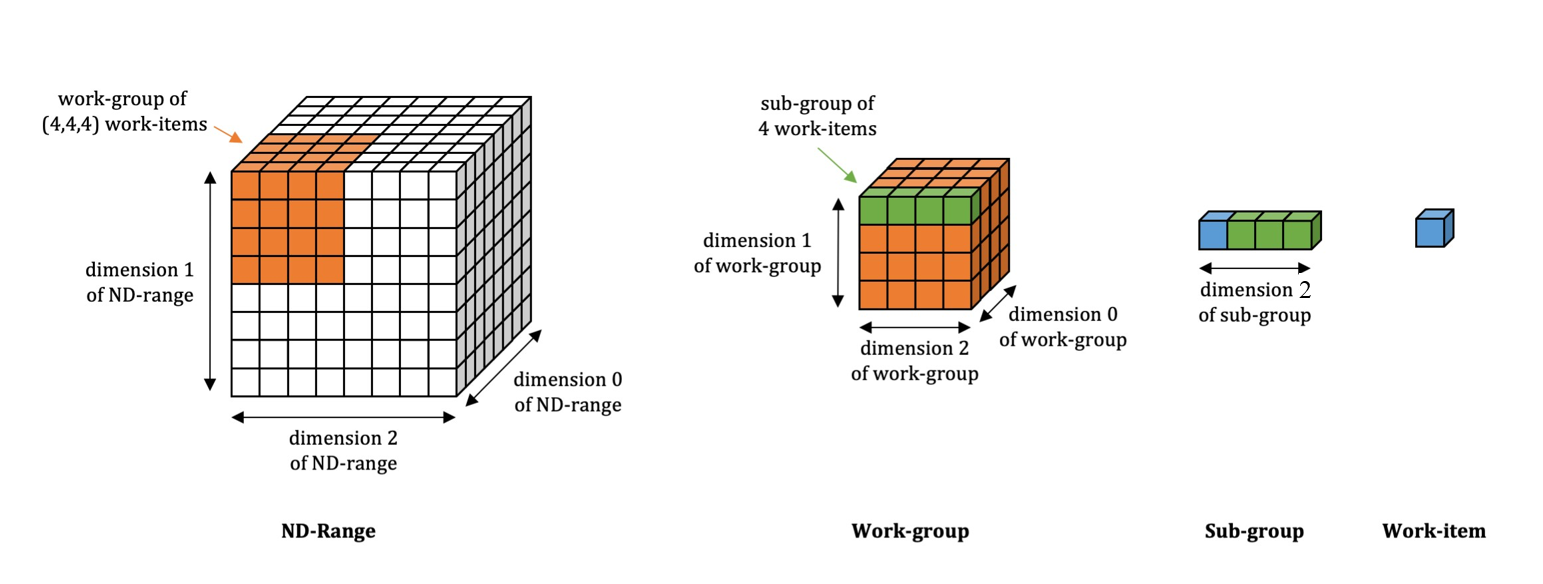
\includegraphics[width=1\textwidth]{figs/sycl/sycl_execution_model.png}
    \caption{At a glance: The SYCL execution model describes relationships between ND-Ranges, work-groups, sub-groups, and work-items.}
    \label{fig:sycl_exec_model}
\end{figure}

% -----------------------------------------------------------------------------
%  Conceptual overview and formal relationships
% -----------------------------------------------------------------------------
\subsection{Conceptual Overview}  Modern accelerator programming models must present the developer with a 
\emph{logical} view of parallel work that is independent of any specific piece of hardware.  SYCL achieves this
by defining a small hierarchy of index spaces.  Each level in the hierarchy provides progressively stronger 
coherence and synchronization guarantees, yet none of them prescribes 
\textit{where} that work will eventually run.  The mapping from logical indices to physical execution resources is
entirely deferred to the run--time or device compiler and is therefore opaque to the application.  In what follows we formalize the four key abstractions exposed by the SYCL execution model and derive a set of identities that will be reused throughout the remainder of this dissertation.

\subsection{Hierarchical Index Spaces}  Let
\[
   \mathbf{G} = (G_x,G_y,G_z) \in \mathbb{N}^3, \qquad
   G_d > 0\quad(d\in\{x,y,z\}) ,
\]
be the \emph{global range}.  It enumerates the total number of logical tasks, or \emph{work--items}, that shall be executed in one kernel invocation.  The associated set of global indices is
\[
    \mathcal{I} \;=\; \{0,\dots,G_x-1\} \times \{0,\dots,G_y-1\} \times \{0,\dots,G_z-1\},
\]
with
\( |\mathcal{I}| = G_x G_y G_z. \)

A second triple
\[
    \mathbf{L} = (L_x,L_y,L_z), \qquad 0 < L_d \le G_d ,
\]
referred to as the \emph{local range}, partitions the ND--Range into disjoint \emph{work--groups}.  Defining
\[
    W_d \;=\; \frac{G_d}{L_d},\qquad d\in\{x,y,z\},
\]
(which implies $G_d \equiv 0\; (\mathrm{mod}\,L_d)$), the set of group indices reads
\[
    \mathcal{W} \;=\; \{0,\dots,W_x-1\} \times \{0,\dots,W_y-1\} \times \{0,\dots,W_z-1\},
\]
with cardinality $|\mathcal{W}|=W_x W_y W_z$.  Each group $w\in\mathcal{W}$ owns exactly
\[
    |\Gamma| \;=\; L_x L_y L_z
\]
work--items that share fast local memory and barrier synchronization.

Within a work--group the implementation may further partition the local index space into \emph{sub--groups} of size $S$:
\[
    S \;=\; |\Sigma|,\quad \Sigma \subseteq \Gamma,\quad 1\le S\le |\Gamma|.
\]
Sub--groups execute in (near) lockstep and admit specialized collective operations, yet their existence and size remain device--specific.  Finally, the singleton element of the hierarchy is the \textbf{work--item}, uniquely addressed by its global id $i=(i_x,i_y,i_z)\in\mathcal{I}$.

The containment relations
\[
    \text{work--item} \;\in\; \text{sub--group} \;\subseteq\; \text{work--group} \;\subseteq\; \text{ND--Range}
\]
hold for every index triple.

\subsection{Abstractness of the Model}  None of the above definitions mention vector widths, cores, or memory banks.  The SYCL execution model is strictly an \emph{index algebra}; it provides (i)~a naming scheme for independent pieces of work, and (ii)~a lattice of synchronization points that the run--time must respect.  Once the tuples $\mathbf{G}$ and $\mathbf{L}$ have been fixed, every additional property of the physical execution, including occupancy, scheduling order, and even whether groups are run concurrently or serially, is an implementation detail.

\subsection*{Notation used from here onward.}  We will exploit the following shorthand throughout the subsequent analysis:
\begin{enumerate}
  \item $|\mathcal{I}|=G_xG_yG_z$ \quad (total work--items),
  \item $|\mathcal{W}|=W_xW_yW_z$ \quad (total work--groups),
  \item $|\Gamma|=L_xL_yL_z$        \quad (work--items per group),
  \item $\langle i_g,i_l\rangle$\quad embodiment of a work--item by its enclosing group index $i_g\in\mathcal{W}$ and its local index $i_l\in\Gamma$.
\end{enumerate}
These identities are purely algebraic and therefore remain valid for \emph{any} SYCL--conformant device.

\paragraph*{From Abstraction to Implementation Strategy.} Next, we translate these concepts into the concrete launch geometries and dependency patterns required by our Monte--Carlo solver.  The forthcoming sections build progressively from global range rounding rules to kernel--specific mappings.
% -----------------------------------------------------------------------------
%  Extended algorithmic description of kernel generation and execution
% -----------------------------------------------------------------------------

\subsection{Basic--Event Sampling Kernels}
\label{subsec:be_kernel}

Each \texttt{Variable} node in layer~$d$ represents an i.i.d.~Bernoulli trial
with success probability~$p\_v\in[0,1]$.  The evaluation of all variables in
a layer is consolidated into 
\emph{one} data--parallel kernel that generates a contiguous block of
bit--packed outcomes:
\begin{enumerate}
  \item \textbf{Parameter staging.}  For every variable~$v$ the solver stores the
        pair $(\text{idx}(v),\,p\_v)$ in host memory, where
        $\text{idx}(v)$ is the global node index.  The list is stable across
        Monte--Carlo iterations and is therefore transferred to device memory
        only once.
  \item \textbf{Contiguous layout.}  A device--side array of $N_{\!v}$
        records, $N_{\!v}$ being the number of variables in the layer, is
        allocated so that the probability field, the bit--packed result buffer
        pointer, and any auxiliary counters are stored in
        \emph{structure--of--arrays} (SoA) form.  The resulting stride--free
        access pattern maximizes global--memory throughput.
  \item \textbf{Kernel configuration.}  Let $T$ denote the total number of
        Bernoulli draws requested by the host run--time (cf.
        Sec.~\ref{sec:bitpack-prob-sampling}).  The global ND--range is chosen
        as $\bigl(\lceil N_{\!v}\rceil,\,B,\,P\bigr)$, mapping each work--item
        to a unique triple $(v,\,b,\,p)$ of variable~$v$, batch index~$b$, and
        bit--pack index~$p$.  The local work--group shape is computed
        adaptively to saturate the target device while respecting hardware
        limits on registers and shared memory.
  \item \textbf{Execution.}  Every work--item initializes a counter--based
        generator (see the Philox discussion in
        Sec.~\ref{sec:bitpack-prob-sampling}), converts the pseudo--random words
        into $\omega$ Bernoulli outcomes via the integer--threshold technique,
        and writes the resulting $w$--bit word to the pre--allocated buffer.
        No inter--item synchronization is required beyond the implicit barrier
        at kernel completion.
\end{enumerate}
The overall cost is $\mathcal{O}(T\,N_{\!v}/\omega)$ arithmetic operations and
$\Theta(T\,N_{\!v}/\omega)$ global writes, making the routine
memory--bandwidth bound only for extremely small~$P$.

\subsection{Gate--Evaluation Kernels}
\label{subsec:gate_kernel}

Gate nodes are logically heterogeneous: AND, OR, XOR, NOT, NAND, NOR, XNOR, and
at--least--$k$ (\texttt{VOT}) gates all feature distinct Boolean semantics yet
share the same interface of reading one or more bit--packed input buffers and
writing a bit--packed output.  To avoid divergent control flow, the solver
instantiates \emph{one specialized kernel per connective type} present in the
current layer.

Consider a set $\mathcal{G}_{\mathrm{type}}$ containing all gates of a single
connective.  Their evaluation proceeds as follows:
\begin{enumerate}
  \item \textbf{Input resolution.}  For every gate $g\in\mathcal{G}$ the lists
        of positive inputs $\mathcal{I}^+(g)$ and negated inputs
        $\mathcal{I}^-(g)$ are resolved to concrete device pointers.  Positive
        and negative buffers are concatenated so that a simple offset marks the
        first negated operand.  The construction is embarrassingly parallel on
        the host and involves no device work.
  \item \textbf{Contiguous block construction.}  Buffers and gate metadata are
        packed into an SoA structure that is tile--aligned for
        coalesced reads.  For at--least--$k$ gates the threshold~$k$ is stored
        alongside the pointer list.
  \item \textbf{Kernel launch geometry.}  Let $N_{\!g}$ be the number of gates
        of the selected type.  An ND--range of
        $\bigl(\lceil N_{\!g}\rceil,\,B,\,P\bigr)$ is created, identical in
        shape to the basic--event kernel so that subsequent layers can reuse
        the same scheduling heuristics.  Within each work--item, Boolean logic
        is applied on a per--bitpack basis without branching:
        \begin{itemize}
          \item \textsc{And}, \textsc{Nand}:  multiple \texttt{\&} reductions
                plus an optional complement.
          \item \textsc{Or}, \textsc{Nor}:   multiple \texttt{|} reductions
                plus an optional complement.
          \item \textsc{Xor}, \textsc{Xnor}: accumulated parity via \texttt{\^{}} operations.
          \item \textsc{Null}, \textsc{Not}: trivial one--input, output, with complement.
          \item \textsc{At--least--$k$}: population counting of the aggregated
                bit--wise sum followed by a threshold comparison implemented
                through native \texttt{popcount} instructions.
        \end{itemize}
  \item \textbf{Dependency guarantees.}  Because all input buffers originate in
        earlier layers, the run--time enforces an event dependency on every
        producing kernel, ensuring visibility of the complete inputs before
        gate evaluation begins.
\end{enumerate}
The bit--parallel operations ensure that the arithmetic intensity is high; the
critical path is dominated by a handful of integer masks and, for
at--least--$k$ gates, one integer addition plus a comparison per input.

\subsection{Dependency--Aware Kernel Scheduling}
\label{subsec:scheduling}

Kernels are submitted to the device queue in strict layer order, yet the
scheduler exploits two orthogonal forms of parallelism:
\begin{enumerate}
  \item \emph{Intra--layer concurrency} --- basic--event sampling and the
        multiple gate kernels of the same layer depend exclusively on the
        previous layer, \emph{not} on one another.  They are therefore eligible
        for concurrent execution subject to device resources.
  \item \emph{Iterative sampling} --- the bit--packed sample space is sliced
        into $T_\text{iter}$ iterations decided by the sample shaper.
        Kernels capturing the same node repeat across iterations and are
        expressed with an explicit iteration counter, enabling the run--time to
        re--use the same compiled binary while varying the random counter seed
        and output offsets.
\end{enumerate}
Dependencies are represented as light--weight events; the host never performs
explicit synchronization inside a layer but relies on the queue to enforce the
partial order.

\subsection{Work--Group Optimization Heuristics}
\label{subsec:wg_optim}

Let $G$ denote the global item count of the kernel at hand and $L_{max}$ the
maximum local size supported by the device along each axis.  The solver
selects a local range $(l_x,l_y,l_z)$ according to
\begin{align*}
  l_x &= min\Bigl(\text{pow2ceil}(G),\,L_{max}\Bigr),\\
  l_y &= min\Biggl(B,\,\frac{L_{max}}{l_x}\Biggr),\\
  l_z &= min\Biggl(P,\,\frac{L_{max}}{l_x l_y}\Biggr),
\end{align*}
which heuristically balances occupancy with register pressure while retaining a
uniform work--item distribution.  The shape is re--evaluated independently for
basic events and gate kernels because $G$ differs across those two categories.

\subsection{Complexity and Scalability}
\label{subsec:complexity}

Assume $|\mathcal{V}|$ variables and $|\mathcal{G}|$ gates in the graph, with
layer depths bounded by $D$.  Let $S=T\,B\,P\,\omega$ be the total number of
Bernoulli trials.
\begin{itemize}
  \item \textbf{Kernel build time.}  All host--side preprocessing runs in
        $\mathcal{O}(|\mathcal{V}|+|\mathcal{G}|)$ memory operations; no search
        structure deeper than a hash map is required.
  \item \textbf{Device execution time.}  Each basic--event kernel performs
        $S$ integer comparisons.  Each gate kernel evaluates $S$ Boolean
        operations whose count is proportional to the fan--in of the gate.
        Hence the total arithmetic complexity is
        $\mathcal{O}\bigl(S\,(1+\overline{\deg})\bigr)$, where
        $\overline{\deg}$ is the average gate fan--in.
  \item \textbf{Parallel scalability.}  Both kernel categories exhibit linear
        speed--up with the number of compute units until either (i)~the global
        launch size no longer saturates the device or (ii)~memory bandwidth
        limits are reached.  Because all kernels are fully independent across
        the $B$ and $P$ dimensions, they scale particularly well on
        multi--tile accelerators.
\end{itemize}

The design therefore provides a clear separation of concerns: depth--first
analysis establishes the dependency structure; kernel generation translates
that structure into homogeneous, vectorizable work; and a light--weight event
system schedules the resulting kernels with minimal host intervention.


\begin{landscape}
\begin{figure}[p]
    \centering
    \includesvg[width=1.15\textheight]{figs/pdag/dag_pass_3.svg}
    \caption{A fully connected Probabilistic-Propositional Directed Acyclic Graph.}
    \label{fig:feedforward_ppdag}
\end{figure}
\end{landscape}


% -----------------------------------------------------------------------------
\section{Kernel-Level Execution Model}
\label{sec:kernel_execution_model}
% -----------------------------------------------------------------------------

\subsection{Coordinate System and Notation}

Let $(G_x,G_y,G_z)\in\mathbb{N}^3$ denote the \emph{global} range supplied to the device and $(L_x,L_y,L_z)$ the \emph{local} (work\,–\,group) range.  We further define
\[
  W_d \;=\; \frac{G_d}{L_d},\qquad d\in\{x,y,z\},
  \quad\text{and}\quad
  W \;=\; W_x W_y W_z ,
\]
where $W_d$ counts work-groups along axis~$d$ and $W$ is the total number of work-groups.  Every work-item within a group is identified by its local id $\ell=(\ell_x,\ell_y,\ell_z)$ with $0\le \ell_d<L_d$.

Unless stated otherwise the following global symbols are used throughout the chapter
\begin{center}
\begin{tabular}{ll}
$V$  & \# basic events (variables)\\
$G$  & \# standard logic gates\\
$A$  & \# at-least-$k$ gates\\
$T$  & Monte-Carlo iterations\\
$B$  & batches per iteration\\
$P$  & bit-packs per batch\\
$\omega$ & bits per pack $=8\cdot\mathrm{sizeof}(\texttt{bitpack\_t})$\\
$N$  & trials per iteration $=B\,P\,\omega$
\end{tabular}
\end{center}

\subsection{Generic Rounding Scheme}

All kernels adopt the \emph{nearest-multiple} rule
\[
   G_d \;=\;
   \Bigl\lceil \frac{Q_d}{L_d} \Bigr\rceil L_d ,\qquad
   Q_d \in \{V,G+A,1\}\times\{B\}\times\{P\},
\]
where $Q_d$ is the problem-specific lower bound listed in Table~\ref{tab:kernel_dimensions}.  This rule guarantees that every logical task is scheduled while respecting the SYCL constraint $G_d\equiv 0 \; (\mathrm{mod}\,L_d)$.

\subsection{Kernel-Specific Mappings}

Each kernel instantiates a surjective mapping
\[
   \Phi : \{0,\dots,G_x-1\}\times\{0,\dots,G_y-1\}\times\{0,\dots,G_z-1\}
          \;\twoheadrightarrow\; \mathcal{S},
\]
where $\mathcal{S}$ is the set of logical sub-tasks it must solve.  We list the mappings succinctly:

\begin{itemize}
  \item \textbf{Basic-event sampling} ($\#\mathcal{S}=VBP$):
        $\,\Phi_{\mathrm{BE}}(i_x,i_y,i_z)=(v=i_x,\;b=i_y,\;p=i_z)$.

  \item \textbf{Standard gate evaluation} ($\#\mathcal{S}=GBP$):
        $\,\Phi_{\mathrm{G}}(i_x,i_y,i_z)=(g=i_x,\;b=i_y,\;p=i_z)$.

  \item \textbf{At-least-$k$ gate evaluation}
        ($\#\mathcal{S}=ABP\omega$):
        $\,i_z = p\,\omega + \lambda$ with $\lambda\in\{0,\dots,\omega-1\}$.  The pair $(b,p)$ indexes the bit-pack, while $\lambda$ singles out a \emph{bit lane}.  One work-group therefore owns a unique triplet $(a,b,p)$ and folds the $\omega$ lanes with a group reduction.

  \item \textbf{Tally accumulation} ($\#\mathcal{S}=VBP$):
        identical to $\Phi_{\mathrm{BE}}$ but with $L_x=1$ such that each group covers exactly one tally node.
\end{itemize}

\subsection{Trial Coverage Guarantee}

Let $\Xi$ be the set of Bernoulli trials processed by a kernel in one iteration.  By construction
\[
   |\Xi|
   \;=\;
   \underbrace{B P \omega}_{\text{trials/ node}}
   \times
   \begin{cases}
     V, & \text{basic-event},\\[2pt]
     G, & \text{standard gate},\\[2pt]
     A, & \text{at-least gate},\\[2pt]
     V, & \text{tally}.
   \end{cases}
\]
Because $\omega$ divides $G_z$ in every case, each trial is owned by exactly one work-item and is executed precisely once.

\begin{table}[t]
  \centering
  \caption{Minimum global dimensions $Q_d$ before round-up.}
  \label{tab:kernel_dimensions}
  \begin{tabular}{lccc}
    \toprule
    Kernel               & $Q_x$              & $Q_y$ & $Q_z$\\
    \midrule
    Basic-event          & $V$                & $B$   & $P$\\
    Standard gate        & $G$                & $B$   & $P$\\
    At-least-$k$ gate    & $A$                & $B$   & $P\omega$\\
    Tally                & $V$                & $B$   & $P$\\
    \bottomrule
  \end{tabular}
\end{table}

\subsection{Work-Group Invariants}

Let $\Gamma$ be a work-group.  For every kernel the following invariant holds inside $\Gamma$:
\[
   \bigl[(\ell_x,\ell_y,\ell_z)\in\Gamma\bigr]
   \;\Longrightarrow\;
   \text{all work-items share the complete set of inputs required to produce one output literal}.
\]
Consequently intra-group communication (reductions, barriers) never crosses logical boundaries, enabling lock-free execution except for the single atomic update in the tally kernel.

\subsection{Complexity per Work-Group}

With $L=L_xL_yL_z$ the number of instructions executed by a group is
\[
  C_{\Gamma}
  \;=\;
  \begin{cases}
    \Theta(\frac{\omega}{4}), & \text{basic-event (bit-packing)},\\
    \Theta(\deg g), & \text{gate of fan-in }\deg g,\\
    \Theta(\deg a + \log \omega), & \text{at-least-}k,\\
    \Theta(L + \log L), & \text{tally popcount + reduction},
  \end{cases}
\]
all independent of $T$ owing to the strict buffering between iterations.

% -----------------------------------------------------------------------------
\section{Bitpacked Random Number Generator}

Monte Carlo simulations, probability evaluations, and other sampling-based procedures benefit greatly from efficient, high-quality \acrfull{rng}s. A large class of modern \acrshort{rng}s are known as \textit{counter-based \acrfull{prng}s}, because they use integer counters (e.g., 32-bit or 64-bit) along with a stateless transformation to produce random outputs. The \emph{Philox} family of counter-based \acrshort{prng}s is a well-known example, featuring fast generation, high period, and good statistical properties. In this section, we discuss the general principles of counter-based \acrshort{prng}s, explain how Philox fits into this paradigm, analyze its complexity, and present a concise pseudocode version of the \(\text{Philox }4\times32\text{-10}\) variant. Subsequently, we detail the bitpacking scheme used to reduce memory consumption when storing large numbers of Bernoulli samples.

A counter-based \acrshort{prng} maps a user-supplied \emph{counter} (plus, optionally, a \emph{key}) to a fixed-size block of random bits via a deterministic function. Formally, if 
\[
  \mathbf{x} \;=\; (x_1, x_2, \ldots, x_k)
\]
is a vector of one or more 32-bit or 64-bit counters, and 
\[
  \mathbf{k} \;=\; (k_1, k_2, \ldots, k_m)
\]
is a key vector, then a counter-based \acrshort{prng} defines a transformation 
\[
   \mathcal{F}(\mathbf{x}, \mathbf{k})
   \;=\;
   (\rho_1, \rho_2, \ldots, \rho_r),
\]
where each \(\rho_j\) is typically a 32-bit or 64-bit output. Different increments of the counter \(\mathbf{x}\) produce different pseudo-random outputs \(\rho_j\). The process is stateless in the sense that advancing the RNG amounts to incrementing the counter (e.g., \(\mathbf{x}\mapsto \mathbf{x} + 1\)).

Compared to older recurrence-based \acrshort{rng}s such as linear congruential generators or the Mersenne Twister, counter-based methods offer more straightforward parallelization, reproducibility across multiple streams, and strong structural simplicity: no internal state must be updated or maintained. This is particularly valuable in distributed Monte Carlo simulations or \acrshort{gpu}-based sampling, where each thread or work-item can be assigned a different counter. Philox constructs its pseudo-random outputs by applying a small set of mixed arithmetic (multiplication/bitwise) rounds to an input \emph{counter} plus \emph{key}. In particular, \(\mathrm{Philox}\,4\times32\text{-10}\) (often shortened to "Philox-4x32-10”) works on four 32-bit integers at a time:
\[
  \mathbf{S} = (S_0, S_1, S_2, S_3),
  \qquad
  \mathbf{K} = (K_0, K_1).
\]
The four elements \(\{S_0, S_1, S_2, S_3\}\) collectively represent the counter, e.g., \((x_0, x_1, x_2, x_3)\). The two key elements \((K_0, K_1)\) are used to tweak the generator's sequence. A single invocation of Philox-4x32-10 transforms \(\mathbf{S}\) into four new 32-bit outputs after ten rounds of mixing. At each round, the algorithm:
\begin{enumerate}
    \item Multiplies two of the state words by fixed "magic constants” to create partial products.
    \item Takes the high and low 32-bit portions of those 64-bit products.
    \item Incorporates the round key to shuffle the words.
    \item Bumps the key by adding constant increments \((\mathrm{W32A} = 0x9E3779B9 \text{ and } \mathrm{W32B} = 0xBB67AE85)\).
\end{enumerate}
After ten rounds, the final \((S_0, S_1, S_2, S_3)\) is returned as the pseudo-random block. A new call to Philox increases the counter \(\mathbf{S}\) by one (e.g., \(S_3 \mapsto S_3 + 1\)) and re-enters the same function. The Philox-4x32-10 algorithm is designed so that each blocking call requires a \emph{constant number} of operations, independent of the size of any prior "state.” Specifically, each round involves:
\[
  \mathcal{O}(1)\;\text{ arithmetic operations},
\]
and there are \(\mathrm{R} = 10\) rounds. Thus, each Philox invocation is asymptotically constant time \(\mathcal{O}(\mathrm{R}) = \mathcal{O}(1)\). The total cost to generate 128 bits (4 words \(\times\) 32 bits) is therefore constant time per call.

\subsection{The 10-round Philox-4x32}
Our implementation follows the standard 10-round approach for generating one block of four 32-bit random words, also called Philox-4x32-10. Let \(M_{\mathrm{A}}=0xD2511F53\), \(M_{\mathrm{B}}=0xCD9E8D57\) be the multipliers, and let \((K_0, K_1)\) be the key which is updated each round by \(\mathrm{W32A}=0x9E3779B9\) and \(\mathrm{W32B}=0xBB67AE85\). The function \(\text{Hi}(\cdot)\) returns the high 32 bits of a 64-bit product, and \(\text{Lo}(\cdot)\) returns the low 32 bits. Because each call produces four 32-bit pseudo-random words, Philox-4x32-10 is particularly convenient for batched sampling. If only a single 32-bit word is needed, one can still call the function and discard the excess words; however, many applications consume all four outputs (e.g., to produce four floating-point variates).

\begin{algorithm}[ht]
  \caption{Philox-4x32-10}\label{alg:philox}
  \begin{algorithmic}[1]
    %------------------------------------------------------------
    \Require Four 32-bit counters $(S_0,S_1,S_2,S_3)$,
            key $(K_0,K_1)$
    \Ensure  Transformed counters $(S_0,S_1,S_2,S_3)$
    %------------------------------------------------------------
    \Statex
    %--------------------- Philox_Round -------------------------
    \Procedure{Philox\_Round}{$(S_0,S_1,S_2,S_3),\,(K_0,K_1)$}
      \State $P_0 \gets M_{\text{A}}\times S_0$ \Comment{64-bit product}
      \State $P_1 \gets M_{\text{B}}\times S_2$ \Comment{64-bit product}
      \State $T_0 \gets \mathrm{Hi}(P_1)\,\oplus\,S_1\,\oplus\,K_0$
      \State $T_1 \gets \mathrm{Lo}(P_1)$
      \State $T_2 \gets \mathrm{Hi}(P_0)\,\oplus\,S_3\,\oplus\,K_1$
      \State $T_3 \gets \mathrm{Lo}(P_0)$
      \State $K_0 \gets K_0 + \mathrm{W32A}$
      \State $K_1 \gets K_1 + \mathrm{W32B}$
      \State \Return $\bigl((T_0,T_1,T_2,T_3),\,(K_0,K_1)\bigr)$
    \EndProcedure
    %------------------- Philox4x32_10 --------------------------
    \Statex
    \Procedure{Philox4x32\_10}{$(S_0,S_1,S_2,S_3),\,(K_0,K_1)$}
      \For{$i \gets 1$ \textbf{to} 10}
        \State $\bigl(S_0,S_1,S_2,S_3),\,(K_0,K_1) \gets$
               \Call{Philox\_Round}{$(S_0,S_1,S_2,S_3),\,(K_0,K_1)$}
      \EndFor
      \State \Return $(S_0,S_1,S_2,S_3)$
    \EndProcedure
  \end{algorithmic}
\end{algorithm}

\subsection{Bitpacking for Probability Sampling}
It takes exactly one bit to represent the outcome of a trial. If these If outcomes are stored naively, each one occupies a full 8-bit byte. Hence, only \( \tfrac{1}{8} \) of the allocated space is used for actual data. By instead packing up to \(w\) indicators into a \(w\)-bit machine word, the memory usage can be reduced by a factor of up to \(8\) (in the simplest scenario of 8-bit groupings). In more general terms:
\[
  \text{Memory usage }M_{\text{naive}}
  \;=\;
  N \times 8\;\text{bits},
  \qquad
  \text{Memory usage }M_{\text{pack}}
  \;=\;
  \left\lceil\frac{N}{w}\right\rceil \,\times\,w\;\text{bits}.
\]
In our implementation, each call to Philox-4x32-10 yields 128 bits of randomness. We use those bits to draw exactly 128 Bernoulli outcomes at once, then combine them into a \(\mathrm{bitpack}\) of two 64-bit integers. For instance, if we choose a batch size of \(4\)-bits to represent four Bernoulli samples in a single chunk, we can:

\begin{enumerate}
    \item Generate a block \(\{r_0, r_1, r_2, r_3\}\) of four 32-bit random integers from Philox.
    \item Convert each \(r_i\) into a uniform \([0,1)\) floating-point value by dividing by \(2^{32}\).
    \item Compare each to the target probability \(p\).
    \item Form a 4-bit integer, each bit set to \(1\) if the corresponding comparison succeeded, or \(0\) otherwise.
\end{enumerate}

Repeating these steps for multiple rounds of 4 bits each can fill a 16-bit or 32-bit \(\mathrm{bitpack}\) variable with many Bernoulli indicators. Then it can be stored into an array at a single index, reducing memory overhead by constant factor of $N$. 

\begin{algorithm}[H]
  \caption{Bit-packing of four Bernoulli samples into a 4-bit block}
  \label{alg:four_bit_pack}
  \begin{algorithmic}[1]
    %------------------------------------------------------------
    \Require Probability $p\in[0,1]$, random 32-bit words $(r_0,r_1,r_2,r_3)$
    \Ensure  4-bit integer bits containing the four Bernoulli draws
    %------------------------------------------------------------
    \Procedure{FourBitPack}{$p,(r_0,r_1,r_2,r_3)$}
      \State bits $\gets 0$
      \For{$i \gets 0$ \textbf{to} 3}
        \State $u_i \gets r_i / 2^{32}$ \Comment{$u_i\in[0,1)$}
        \If{$u_i < p$}
            \State $b_i \gets 1$
        \Else
            \State $b_i \gets 0$
        \EndIf
        \State bits $\gets$ bits $\mid (b_i \ll i)$ 
               \Comment{set bit $i$ to $b_i$}
      \EndFor
      \State \Return bits
    \EndProcedure
  \end{algorithmic}
\end{algorithm}

In this procedure, \(\Vert\) denotes a bitwise OR, and \(\ll\) denotes a left shift. One then repeats the above call to accumulate multiple 4-bit blocks (e.g., for a total of 16 bits, one calls FourBitPack four times and merges the results with the appropriate shifts).
\chapter{Tallying Layer Outputs}
\label{sec:tally_kernel}

At every Monte-Carlo iteration the simulator produces, for each logic node
\(v\in \mathcal{V}\), a bit-packed buffer encoding
\[
  \mathbf{Y}_v^{(t)}
  \;=\;
  \bigl(y_{v,1}^{(t)}, y_{v,2}^{(t)},\dots, y_{v,N}^{(t)}\bigr)
  \in\{0,1\}^N,
  \quad t = 1,\dots,T,
\]
where \(N\!=\!B\!\times\!P\!\times\!\omega\) is the number of Bernoulli trials
per Monte-Carlo \emph{iteration}:
\begin{itemize}
    \item \(B\) - number of \emph{batches},
    \item \(P\) - bit-packs per batch,
    \item \(\omega\!=\!8\cdot\mathrm{sizeof}(\text{bitpack\_t})\) - bits per pack.
\end{itemize}
Because the buffers are overwritten at the next iteration, a
separate \emph{tally layer} accumulates summary statistics that persist for the
entire simulation.  The present section formalizes that process and outlines
an implementation-agnostic, data-parallel algorithm that realizes it on modern
accelerators.

\section{Statistical Objectives}
\label{subsec:tally_objective}

For every node \(v\) we wish to estimate, after \(T\) Monte-Carlo iterations,

\[
  \widehat{p}_v
  \;=\;
  \frac{1}{T\,N}
  \sum_{t=1}^{T}\sum_{j=1}^{N} y_{v,j}^{(t)}
  \;=\;
  \frac{s_v}{T\,N},
  \qquad
  s_v \;=\; \text{total \# of one-bits observed for node \(v\)}.
\]

Under the usual independence assumptions, the sampling distribution of
\(\widehat{p}_v\) is asymptotically
\[
\mathcal{N}\!\bigl(p_v,\,
  \tfrac{p_v(1-p_v)}{T\,N}\bigr)
\]
Hence

\[
  \widehat{\sigma}_v
  \;=\;
  \sqrt{\frac{\widehat{p}_v\,(1-\widehat{p}_v)}{T\,N}}
\]

is an unbiased estimator of the standard error, giving the
\((1-\alpha)\)\,--\,level normal confidence interval

\[
  \bigl[
    \widehat{p}_v - z_{1-\alpha/2}\,\widehat{\sigma}_v,\;
    \widehat{p}_v + z_{1-\alpha/2}\,\widehat{\sigma}_v
  \bigr],
  \qquad
  z_{1-\alpha/2}\in\{1.96,\,2.58,\dots\}.
\]

The tally routine therefore needs to maintain only the scalar
\(s_v\) while the simulation is running; the derived statistics can be updated
in-place whenever a user requests intermediate results or at a fixed cadence.

\section{Parallel Accumulation Algorithm}

The accumulation kernel is invoked on a three-dimensional
\texttt{nd\_range}, chosen such that
\[
  \begin{aligned}
    \text{global}_x &\;\ge\; V,\\
    \text{global}_y &\;\ge\; B,\\
    \text{global}_z &\;\ge\; P.
  \end{aligned}
\]
Work-item \((i_x,i_y,i_z)\) is responsible for \emph{exactly one} bit-pack:
\[
  \text{node  } v=i_x,\quad
  \text{batch } b=i_y,\quad
  \text{pack  } p=i_z.
\]

\vspace{4pt}
\noindent
\textbf{Local workflow of a work-item}
\begin{enumerate}
    \item Load the \(p^{\text{th}}\) bit-pack of batch \(b\) from
          \texttt{buffer}.
    \item Compute \(c=\mathrm{popcount}(\text{bitpack})\).
    \item Reduce the \(c\)'s belonging to the same work-\emph{group} in
          shared memory (tree reduction or \texttt{reduce\_over\_group}).
    \item One designated leader performs
          \(\texttt{atomic\_add}(\texttt{num\_one\_bits},\,\text{group\_sum})\).
\end{enumerate}

The reduction ensures only one atomic operation per group, greatly reducing
contention when \(P\) is large.

We present platform-neutral pseudocode that encapsulates the above logic while remaining agnostic to the underlying API. After each Monte-Carlo iteration the host enqueues \textsc{TallyKernel} with a
fresh \texttt{iteration} counter.  When either (i)~a user requests
intermediate statistics or (ii)~a pre-set reporting interval is reached,
the host reads back \texttt{num\_one\_bits} and executes the purely
serial routine shown in Algorithm~\ref{alg:update_stats}.

\begin{algorithm}[H]
\caption{Post-processing of a single node's tally}
\label{alg:update_stats}
\begin{algorithmic}[1]
  \Require
    \(s\) - total one-bits,
    \(T\), \(B\), \(P\), \(\omega\) - run parameters
  \Ensure
    \(\widehat{p}\), \(\widehat{\sigma}\), two symmetric CIs
  \State $N\gets B\cdot P\cdot\omega$
  \State $\widehat{p}\gets s / (T\,N)$
  \State $\widehat{\sigma}\gets
          \sqrt{\widehat{p}(1-\widehat{p})/(T\,N)}$
  \For{\textbf{each} $z\in\{1.96,\,2.58\}$}
      \State $\text{CI}\gets
        \bigl[\max(0,\widehat{p}-z\widehat{\sigma}),
              \min(1,\widehat{p}+z\widehat{\sigma})\bigr]$
  \EndFor
\end{algorithmic}
\end{algorithm}

The above normal approximation is valid provided \(T\,N\widehat{p}\)
and \(T\,N(1-\widehat{p})\) both exceed roughly 10; otherwise an exact
Clopper-Pearson interval can be substituted with no change to the running
sum logic.

\section{Correctness and Complexity}

\textbf{Work-item cost.}
Each work-item performs one \(\mathrm{popcount}\) and
participates in an \(O(\log L)\) intra-group reduction
(\(L\!=\!\text{local\_range}\)), yielding an overall
\(O(\log L)\) instruction count.

\textbf{Global cost.}
The total number of work-items launched per iteration is
\(V\cdot B\cdot P\).  Because each bit-pack contains \(\omega\) Bernoulli
trials, the cost \emph{per trial} shrinks as \(\omega^{-1}\).

\textbf{Memory traffic.}
Every work-item reads exactly one machine word and no writes occur except
the single atomic addition per work-group.  Hence the algorithm is
memory-bandwidth bound only at extremely low arithmetic intensity
(\(P\approx 1\)).

\textbf{Linear scalability.}
All tally nodes are independent.  Increasing \(V\) therefore scales the total
runtime linearly until either (i)~the device saturates its occupancy or
(ii)~atomic contention becomes non-negligible; the group-level reduction
mitigates the latter.

The design therefore provides a clear separation of concerns: depth--first
analysis establishes the dependency structure; kernel generation translates
that structure into homogeneous, vectorizable work; and a light--weight event
system schedules the resulting kernels with minimal host intervention.

% -----------------------------------------------------------------------------
%  Extended implementation-oriented discussion (matches the realised kernel)
% -----------------------------------------------------------------------------

\section{Work--Group Geometry and Synchronization}
\label{subsec:tally_geometry}

The three--dimensional launch geometry \((v,\,b,\,p)\) outlined in
Sec.~\ref{subsec:tally_objective} is refined in the implementation to minimize
both occupancy loss and atomic contention.  A crucial design choice is to fix
\emph{local}~\(x=1\), thereby dedicating one work--group to exactly one tally
node~\(v\).  The remaining two dimensions then tile the \((b,p)\)--plane with a
rectangular block of size
\[
  \bigl(1,\,l_y,\,l_z\bigr),
  \qquad l_y\cdot l_z\le L_{\max},
\]
where \(L_{\max}\) is the device--specific upper bound on the total work--group
size.  Provided \(l_y\!\ge\!B\) and \(l_z\!\ge\!P\), only \emph{one} group is
dispatched per tally and per iteration, guaranteeing that the reduction of
Step~3 and the atomic addition of Step~4 in
Sec.~\ref{sec:tally_kernel} execute exactly once.  Should resource pressure
force \(l_y< B\) or \(l_z< P\), multiple groups are launched and the atomic
update is replicated; correctness is preserved by the commutativity of
addition, but the repeated work incurs a small overhead.  The occupancy model
therefore trades a moderate loss in parallelism for deterministic behavior and
reduced synchronization cost.

A relaxed memory order is sufficient for the atomic accumulator because the
kernel guarantees \emph{program order} between the intra--group reduction and
the atomic~\texttt{fetch\_add}.  No additional fences are required, and the
resulting implementation maps efficiently to both discrete and integrated
\acrshort{gpu}s.

\section{Incremental Update of Derived Statistics}
\label{subsec:tally_stats_refresh}

While Monte--Carlo sampling proceeds, applications often request intermediate
probability estimates~\(\widehat{p}_v^{(t)}\) before the total budget~\(T\) is
exhausted.  Recomputing \(\widehat{p}_v\) and
\(\widehat{\sigma}_v\) from scratch would require a host round--trip for every
sampled bit.  Instead, the tally layer maintains two scalars per node:
\(s_v\) (total one--bits) and \(n_v\) (total bits processed).  After each
completed iteration the host merely increments \(n_v\gets n_v + N\) and leaves
\(s_v\) to the device kernel.  Whenever a refresh is requested the statistics
are updated via
\[
  \widehat{p}_v\;=\;\frac{s_v}{n_v},
  \qquad
  \widehat{\sigma}_v\;=\;\sqrt{\frac{\widehat{p}_v(1-\widehat{p}_v)}{n_v}},
\]
which costs \(\mathcal{O}(V)\) host--side arithmetic and no device work.  In
practice the refresh cadence is set adaptively: frequent updates early in the
run aid variance monitoring, whereas late--stage updates can be spaced further
apart because the relative change in \(\widehat{p}_v\) diminishes as
\(n_v\to T\,N\).

\section{Convergence Diagnostics and Stopping Rules}
\label{subsec:tally_convergence}

Two families of diagnostics leverage the quantities already maintained by the
tally kernel:
\begin{enumerate}
  \item\textbf{Relative half--width criterion.}  Define the
        half--width of the \((1-\alpha)\)--level interval as
        \(h_v= z_{1-\alpha/2}\,\widehat{\sigma}_v\).  The run may be terminated
        for node~\(v\) once \(h_v/\widehat{p}_v\le \varepsilon\), where
        \(\varepsilon\) is a user--supplied tolerance.  Because both
        \(\widehat{\sigma}_v\) and \(\widehat{p}_v\) are inexpensive to update,
        the test incurs negligible overhead.
  \item\textbf{Sequential Wald test.}  When the goal is to decide whether
        \(p_v\) exceeds a safety threshold~\(p_0\), one may adopt the
        sequential probability ratio test with boundaries derived from
        \(s_v\) and \(n_v\).  The tally structure already provides the minimal
        sufficient statistics, so the host evaluates the Wald condition after
        every refresh with no additional device interaction.
\end{enumerate}
Because the diagnostics rely solely on \(s_v\) and \(n_v\), no modification to
the kernel is needed; all logic resides in a lightweight host callback.

\section{Implementation Cost Model}
\label{subsec:tally_cost_model}

Let \(C_{\mathrm{pc}}\) denote the latency of a hardware popcount and
\(C_{\mathrm{rd}}(l)\) the latency of a tree reduction over \(l\) work--items.
The wall--clock time per iteration is approximated by
\[
  T_{\text{iter}} \;\approx\;
  (C_{\mathrm{pc}} + C_{\mathrm{mem}})\,VBP +
  C_{\mathrm{rd}}(l_y l_z)\,\frac{VBP}{l_y l_z}
  + C_{\mathrm{atomic}}\,\frac{VBP}{l_y l_z},
\]
where \(C_{\mathrm{mem}}\) and \(C_{\mathrm{atomic}}\) are the per--word memory
and atomic latencies, respectively.  The model highlights two regimes:
\begin{itemize}
  \item\emph{Arithmetic bound}: when \(P\gg 1\) and the popcount throughput
        saturates the execution units, the first term dominates and scaling is
        limited by instruction bandwidth.
  \item\emph{Memory bound}: when \(P\approx 1\) the workload collapses to a
        single read per work--item; the kernel becomes memory bandwidth--
        limited as predicted in Sec.~\ref{subsec:tally_objective}.
\end{itemize}


\section{Numerical Robustness}
\label{subsec:tally_numerics}

All accumulators operate in integer arithmetic, thereby eliminating rounding
error in \(s_v\).  Derived quantities computed in double precision satisfy
\(\lvert\widehat{p}_v - s_v/n_v\rvert < 2^{-53}\), well below any practical
error criterion for reliability analysis.  Clamping the confidence interval
bounds to~\([0,1]\) prevents pathological estimates when either \(s_v=0\) or
\(s_v=n_v\) in early iterations.

% -----------------------------------------------------------------------------
\section{Relation to the Global Execution Model}
\label{subsec:tally_exec_relation}

The specialised geometry adopted in Section~\ref{subsec:tally_geometry} is a direct instantiation of the rules formalised in Section~\ref{sec:kernel_execution_model}.  Choosing $L_x=1$ enforces the work\,–\,group invariant whereby a group owns exactly one tally node while still satisfying
\[
   G_x \;=\; \Bigl\lceil \frac{V}{L_x} \Bigr\rceil L_x \;=\; V ,
\]
so no over-provisioning occurs along the $x$-axis.  The remaining dimensions follow the generic rounding scheme with $(Q_y,Q_z)=(B,P)$, thus preserving the one-to-one correspondence between work-items and bit-packs established in Section~\ref{sec:kernel_execution_model}.

\chapter{Preliminary Benchmarks on Arialia Fault Trees}
\subsection{Runtime Environment and Benchmarking Setup}
\label{subsec:runtime_environment}

All experiments were performed on a consumer-grade desktop provisioned with an NVIDIA\textsuperscript{\textregistered} GeForce GTX~1660~SUPER graphics card (1{,}408~CUDA cores, 6\,\acrshort{gb} of dedicated GDDR6 memory) and a 10th-generation Intel\textsuperscript{\textregistered} Core\textsuperscript{TM}~i7-10700 \acrshort{cpu} (2.90\,GHz base clock, with turbo-boost and hyperthreading enabled). The code implementation relies on \acrshort{sycl} using the AdaptiveCpp (formerly HipSYCL) framework, which employs an LLVM based runtime and \acrfull{jit} kernel compilation.

\subsubsection*{Monte Carlo Sampling Strategy}
Each fault tree model was evaluated through a single pass (one iteration), generating as many Monte Carlo samples as would fit into the \acrshort{gpu}'s 6\,\acrshort{gb} memory. A 64-bit counter-based Philox4x32x10 random number generator was applied in parallel to produce the basic-event realizations. Note, with the exception of \texttt{das9205}, for which 5 passes were performed (in $\approx 0.96$ seconds), all inputs were quantified using just one pass. We specifically chose \texttt{das9205} since its overall event probability is quite low, and requires many naive Monte Carlo samples.

\subsubsection*{Bit-Packing and Data Types}
To reduce memory usage and increase vectorized throughput, every batch of Monte Carlo results was bit-packed into 64-bit words. Accumulated tallies of successes or failures were stored as 64-bit integers, while floating-point calculations (e.g., probability estimates) used double precision (64-bit floats). These design decisions are intended to maintain numerical consistency and make use of native hardware operations (such as population-count instructions for threshold gates).

\subsubsection*{Execution Procedure}
Upon launching the application, the enabling overhead (host-device transfers, \acrshort{jit} compilation, and kernel configuration) was included in the total wall-clock measurement. Each benchmark was compiled at the \texttt{-O3} optimization level to ensure efficient instruction generation. Every experiment was repeated at least five times, and measured runtimes were averaged to reduce the impact of transient background processes or scheduling variations on the host system.

\subsection{Assumptions and Constraints}
The primary objective was to gauge runtime across a set of fault trees that vary widely in size, logic complexity, and probability ranges within a typical Monte Carlo integration workflow. The experiments assume independent operation of the test machine, with no significant other processes contending for \acrshort{gpu} or \acrshort{cpu} resources. All sampling took place within a single pass, so the measured wall times incorporate initial kernel launches, memory copies, and statistical collection of gate outcomes. No specialized forms of hardware optimization beyond the data-parallel approach (e.g., pinned memory or asynchronous streams) were used.

\subsection{Comparative Accuracy \& Runtime}

Table~\ref{tab:canopy-logp-mae} and Figure~\ref{fig:canopy_rel_error_plot} summarize the accuracy of three approximate quantification methods \acrfull{rea}, \acrfull{mcub}, and our \acrshort{gpu}-accelerated Monte Carlo by listing each approach's mean relative error in the log-probability (\(\log p\)) domain, alongside the total MC samples and runtime. Although each fault tree exhibits its own complexities, several broad trends emerge:

\begin{enumerate}
    \item \textbf{\acrshort{rea} accuracy strongly depends on the \emph{actual} top-event probability.}
    \begin{itemize}
        \item For trees with very low-probability failures (e.g., \texttt{baobab1}, \texttt{das9202}, \texttt{isp9605}), where individual component failures rarely coincide, \acrshort{rea}'s mean error often remains near or below \(10^{-2}\) in log space. This indicates that summing only the first-order minimal cut sets--assuming higher-order intersections contribute negligibly--can be valid when the system is indeed dominated by single-component or few-component events.
        \item However, for fault trees with moderate or higher top-event probabilities (\(\gtrsim 10^{-2}\)), \acrshort{rea}'s inaccuracy tends to grow (for instance, up to \(10^{-1}\) in \texttt{edf9203}, \texttt{edf9204}, and \texttt{edfpa15b}). In these cases, ignoring the overlap of multiple cut sets leads to a visible systematic error.
    \end{itemize}

    \item \textbf{Min-Cut Upper Bound (\acrshort{mcub}) often mirrors \acrshort{rea} but with exaggerated errors in certain overlapping cut configurations.}
    \begin{itemize}
        \item In many models (e.g., \texttt{cea9601}, \texttt{baobab3}, \texttt{das9601}), \acrshort{mcub} closely tracks \acrshort{rea}, suggesting that higher-order combinations remain negligible in those systems.
        \item Yet, in a few cases involving heavy cut-set overlap (e.g., \texttt{das9209}, row~14), \acrshort{mcub} soars to a mean log-probability error of \(\sim 17\), dwarfing \acrshort{rea} or Monte Carlo. This highlights the well-known pitfall: if multiple cut sets are not genuinely ``rare'' and substantially overlap, the union bound becomes extremely loose.
    \end{itemize}

    \item \textbf{Monte Carlo yields more consistent and often dramatically lower numerical errors for most moderate- to high-probability top events.}
    \begin{itemize}
        \item For example, in \texttt{das9201} (row~6) and \texttt{edf9203} (row~19), the Monte Carlo error is well below \(10^{-3}\), whereas both \acrshort{rea} and \acrshort{mcub} can exceed \(10^{-1}\). In these situations, ignoring or bounding higher-order intersections proves inadequate, while direct sampling naturally captures all overlaps.
        \item However, for fault trees with extremely small top-event probabilities, Monte Carlo's variance can become harder to control. For instance, some rows (\texttt{das9204}, \texttt{das9205}, \texttt{isp9605}, \texttt{isp9607}) show that roughly \(10^{8}\)--\(10^{9}\) samples are required to constrain the error within a few tenths in \(\log p\). Those entries either exhibit a slightly higher Monte Carlo error than \acrshort{rea}/\acrshort{mcub} or demonstrate that we needed a disproportionately large sample count (and thus more runtime) to compete with simple rare-event approximations.
    \end{itemize}

    \item \textbf{Sampling scale and runtime remain surprisingly feasible, even for up to \(10^{9}\) draws.}
    \begin{itemize}
        \item Despite some test cases sampling in the hundreds of millions or billions, runtimes remain \(\approx 0.2\)--\(0.3\)~s for most fault trees, rarely exceeding 1~s (see, for instance, row~10 with 3.3~B samples and \(\sim 0.96\)~s). This indicates that the bit-packed, data-parallel Monte Carlo engine is highly optimized, making large-sample simulation a viable alternative to purely analytical approaches for many real-world PRA problems.
        \item By contrast, the bounding methods (\acrshort{rea} and \acrshort{mcub}) typically run in negligible time but deliver inconsistent accuracy depending on each tree's structure. In practice, a hybrid strategy may emerge: apply bounding methods for quick estimates, then selectively invoke large-sample Monte Carlo for trees or subsections where the bounding approximation diverges.
    \end{itemize}

    \item \textbf{Omitted or Extreme Cases.}
    \begin{itemize}
        \item Rows where Monte Carlo entries are missing (e.g., \texttt{das9209} and \texttt{edf9206}) indicate difficulty in converging to a useful estimate within a fixed iteration budget. Conversely, \acrshort{mcub} shows erratic jumps in some of those same cases, underlining the fact that both bounding and sampling approaches can struggle in certain outliers.
        \item Model \texttt{nus9601} (row~43) lacks all three error columns since no reference solution was available, reflecting a scenario where direct verification remains pending or inapplicable. Nevertheless, the completion time of \(\sim 0.29\)~s for a partial exploration suggests that the structural overhead of large fault trees can still be handled efficiently.
    \end{itemize}
\end{enumerate}

These results affirm that Monte Carlo methods, when equipped with high throughput sampling, can achieve the most robust accuracy across a broader spectrum of top-event probabilities, particularly in configurations where standard cut set approximations fail to capture significant event dependencies. At the same time, rare-event with exceptionally small probabilities can pose challenges for naive sampling, revealing the potential need for adaptive variance-reduction techniques or partial enumerations. In practice, analysts may combine bounding calculations (\acrshort{rea}/\acrshort{mcub}) for quick screening or preparatory checks, then use hardware-accelerated Monte Carlo to refine those domains most susceptible to underestimation or overestimation by simpler approximations. Alternatively, for very large models, where exact solutions may be unavailable, data-parallel Monte Carlo can still estimate event probabilities without building minimal cut sets. 

% \begin{landscape}
\sisetup{ 
  scientific-notation = true,
  table-format        = 1.2e-2,
  round-mode          = places,
  round-direction     = up,
  round-precision     = 2,
  group-separator     = {,},
  group-minimum-digits= 4,
  table-text-alignment=center,
  table-number-alignment = center,
}
\begin{longtable}{@{}l
                     l
                     S
                     S
                     S
                     S[table-format=1.1e-2,round-precision=1]
                     S[scientific-notation=false, table-format=1.3]@{}}
\caption{Relative error (Log-probability), \acrfull{dpmc} vs \acrfull{mcub} and \acrfull{rea}.}
\label{tab:canopy-logp-mae}\\
\toprule
\textbf{\#} &
  \makecell{\textbf{Fault}\\\textbf{Tree}} &
  \multicolumn{3}{c}{\textbf{Relative Error $\left| \log_{10}\left(\frac{P_{\text{approx}}}{P_{\text{exact}}}\right) \right|$}} &
  \textbf{Samples} &
  \textbf{Runtime (\si{\second})} \\
\cmidrule(lr){3-5}
& & \textbf{\acrshort{rea}} & \textbf{\acrshort{mcub}} & \textbf{\acrshort{dpmc}} & & \\
\midrule
\endfirsthead
\multicolumn{7}{c}{\textit{Table 12.1: Relative Error (Log-Probability), \acrshort{dpmc} vs \acrshort{mcub}, \acrshort{rea}.}}\\
\toprule
\textbf{\#} &
  \makecell{\textbf{Fault}\\\textbf{Tree}} &
  \multicolumn{3}{c}{\textbf{Relative Error $\left| \log_{10}\left(\frac{P_{\text{approx}}}{P_{\text{exact}}}\right) \right|$}} &
  \textbf{Samples} &
  \textbf{Runtime (\si{\second})} \\
\cmidrule(lr){3-5}
& & \textbf{\acrshort{rea}} & \textbf{\acrshort{mcub}} & \textbf{\acrshort{dpmc}} & & \\
\midrule
\endhead
\bottomrule
\endfoot
%
\endlastfoot
%
\textbf{1}  & baobab1  & 1.45156E-04 & 1.45156E-04 & 7.61880E-03                         & 2.5E+08 & 0.262 \\
\textbf{2}  & baobab2  & 6.48628E-03 & 6.34705E-03 & 1.54436E-03 & 2.5E+08 & 0.209 \\
\textbf{3}  & baobab3  & 1.21509E-02 & 1.16701E-02 & 2.24843E-04 & 2.4E+08 & 0.259 \\
\textbf{4}  & cea9601  & 9.36195E-02 & 9.32207E-02 & 2.41802E-03 & 1.2E+08 & 0.262 \\
\textbf{5}  & chinese  & 1.08742E-02 & 1.06354E-02 & 2.14601E-03 & 9.4E+08 & 0.277 \\
\textbf{6}  & das9201  & 1.26649E-01 & 1.22765E-01 & 5.49963E-05 & 2.3E+08 & 0.279 \\
\textbf{7}  & das9202  & 7.72743E-05 & 2.57596E-05 & 1.20232E-04                         & 5.2E+08 & 0.295 \\
\textbf{8}  & das9203  & 3.59019E-02 & 3.55935E-02 & 2.31768E-04 & 5.2E+08 & 0.292 \\
\textbf{9}  & das9204  & 1.68086E-01 & 1.68087E-01 & 1.13495E-01 & 6.1E+08 & 0.292 \\
\textbf{10} & das9205  & 9.63825E-02 & 9.63725E-02 & 2.76190E-02 & 3.3E+09 & 0.958 \\
\textbf{11} & das9206  & 5.43561E-02 & 8.89660E-04 & 3.51548E-04 & 2.0E+08 & 0.269 \\
\textbf{12} & das9207  & 1.18486E-01 & 2.45492E-02 & 1.36519E-04 & 9.5E+07 & 0.282 \\
\textbf{13} & das9208  & 4.12808E-02 & 3.81968E-02 & 9.34017E-05 & 2.5E+08 & 0.307 \\
\textbf{14} &
  das9209 &
  2.11242E-02 &
  1.70245E+01 &
   &
   &
   \\
\textbf{15} & das9601  & 5.29285E-02 & 5.19122E-02 & 6.67174E-04 & 1.1E+08 & 0.256 \\
\textbf{16} & das9701  & 5.02804E-02 & 3.37565E-02 & 6.22978E-04 & 2.3E+07 & 0.273 \\
\textbf{17} & edf9201  & 1.48012E-01 & 5.36182E-02 & 2.88906E-04 & 1.8E+08 & 0.315 \\
\textbf{18} & edf9202  & 1.07181E-01 & 6.05976E-03 & 4.53900E-04 & 7.8E+07 & 0.271 \\
\textbf{19} & edf9203  & 2.22146E-01 & 1.17293E-01 & 3.27993E-04 & 8.0E+07 & 0.302 \\
\textbf{20} & edf9204  & 2.79531E-01 & 1.05591E-01 & 1.31416E-04 & 8.7E+07 & 0.298 \\
\textbf{21} & edf9205  & 9.94339E-02 & 4.46260E-02 & 5.60146E-05 & 1.9E+08 & 0.284 \\
\textbf{22} & edf9206  & 6.98797E-03 & 7.07775E-03 &                                    &        &      \\
\textbf{23} & edfpa14b & 1.85574E-01 & 9.15983E-02 & 1.04767E-03 & 9.4E+07 & 0.267 \\
\textbf{24} & edfpa14o & 1.86482E-01 & 9.18665E-02 & 3.39049E-04 & 9.8E+07 & 0.275 \\
\textbf{25} & edfpa14p & 3.40010E-02 & 1.66283E-02 & 5.35099E-04 & 2.1E+08 & 0.294 \\
\textbf{26} & edfpa14q & 1.85609E-01 & 9.15366E-02 & 3.33292E-04 & 9.6E+07 & 0.282 \\
\textbf{27} & edfpa14r & 2.48088E-02 & 2.09729E-02 & 9.33865E-04 & 2.1E+08 & 0.294 \\
\textbf{28} & edfpa15b & 2.16329E-01 & 9.37065E-02 & 4.67881E-04 & 1.1E+08 & 0.283 \\
\textbf{29} & edfpa15o & 2.16502E-01 & 9.37627E-02 & 4.06846E-05 & 1.1E+08 & 0.282 \\
\textbf{30} & edfpa15p & 2.52568E-02 & 1.00382E-02 & 3.54344E-04 & 2.6E+08 & 0.299 \\
\textbf{31} & edfpa15q & 2.16329E-01 & 9.37065E-02 & 6.74736E-04 & 1.1E+08 & 0.284 \\
\textbf{32} & edfpa15r & 1.94693E-02 & 1.62668E-02 & 4.04924E-04 & 2.5E+08 & 0.290 \\
\textbf{33} & elf9601  & 1.98107E-02 & 8.08925E-05 & 7.86600E-05 & 2.3E+08 & 0.274 \\
\textbf{34} & ftr10    & 1.22076E-01 & 9.27268E-04 & 1.54844E-04 & 2.1E+08 & 0.297 \\
\textbf{35} & isp9601  & 8.08392E-02 & 6.63074E-02 & 1.13264E-04 & 1.8E+08 & 0.271 \\
\textbf{36} & isp9602  & 1.74572E-02 & 1.47782E-02 & 1.35280E-03 & 2.3E+08 & 0.281 \\
\textbf{37} & isp9603  & 3.82337E-02 & 3.74815E-02 & 3.82344E-03 & 2.7E+08 & 0.278 \\
\textbf{38} & isp9604  & 1.20889E-01 & 8.14313E-02 & 1.88665E-04 & 1.4E+08 & 0.280 \\
\textbf{39} & isp9605  & 6.57344E-03 & 6.57032E-03 & 2.93472E-02                         & 5.0E+08 & 0.262 \\
\textbf{40} & isp9606  & 2.27811E-02 & 1.18983E-02 & 1.30307E-04 & 3.4E+08 & 0.289 \\
\textbf{41} & isp9607  & 2.38880E-02 & 2.38880E-02 & 1.28136E-01                         & 3.8E+08 & 0.282 \\
\textbf{42} & jbd9601  & 1.22001E-01 & 1.35343E-02 & 1.08116E-04 & 5.7E+07 & 0.279 \\
\textbf{43} & nus9601  &            &            &                                    & 1.6E+07 & 0.289 \\* \bottomrule
\end{longtable}
% \end{landscape}


\subsection{Memory Consumption}

As mentioned previously, the memory was set to the maximum allocatable 6\acrshort{gb}, constrained by the NVIDIA GTX 1660 SUPER \acrshort{gpu}'s \acrshort{vram}. Figure \ref{fig:canopy_rel_error_plot_1} plots the actual consumed memory, as a function of \acrshort{pdag} input size and total number of bits sampled per node (gate or basic-event) per pass. Since there are multiple types of preprocessing steps, all of which affect the final size of the pruned \acrshort{pdag}, those have been plotted in Figure \ref{fig:canopy_rel_error_plot_2} for completeness. Since the nature of the actual pruning logic is not being benchmarked here, we named these v1, v2, v3 respectively. The key takeaways are that while some trees are more compressible than others, nearly all computations were performed by saturating available \acrshort{vram}. As a zoomed out version of Figure \ref{fig:canopy_rel_error_plot_1} , Figure \ref{fig:sampled_bits_mem} projects trends for the sampled bits count, as a function of model size, for varying amounts of available \acrshort{ram}.
\begin{landscape}
\begin{figure}[p]
    \centering
    \includesvg[width=1.38\textheight]{task_III/canopy/plots/rel_error.svg}
    \caption{Relative error (Log-probability) for \acrfull{dpmc} vs \acrfull{mcub} and \acrfull{rea}}
    \label{fig:canopy_rel_error_plot}
\end{figure}
\end{landscape}


\begin{landscape}
\begin{figure}
    \centering
    \begin{subfigure}[t]{0.663\textwidth}
        \centering
        \includesvg[width=\linewidth]{task_III/canopy/plots/mem_allocation_lines_zoom.svg}
        \caption{Sampled Bits per Event per Iteration}
        \label{fig:canopy_rel_error_plot_1}
    \end{subfigure}
    \hfill
    \begin{subfigure}[t]{0.659\textwidth}
        \centering
        \includesvg[width=\linewidth]{task_III/canopy/plots/mem_allocation_lines_zoom_all.svg}
        \caption{Sampled Bits per Event per Iteration}
        \label{fig:canopy_rel_error_plot_2}
    \end{subfigure}
    \caption{Comparison of sampled bits per event per iteration.}
\end{figure}
\end{landscape}

\begin{figure}
    % \centerline{}
    \includesvg[width=0.95\textwidth]{task_III/canopy/plots/mem_allocation_lines_lg.svg}
    \caption{Sampled bits per event per iteration}
    \label{fig:sampled_bits_mem}
\end{figure}
\section{Limitations}

\section{Transformations}
\subsection{Knowledge Compilation}
Casting \acrshort{pra} model as \acrshort{pdag} allows to view the model a set of boolean propositional statements. Thus, any question that can be asked about the system, can be seen as a general reasoning (queries or transformations) over the knowledge base, defined by the propositional statements. A common approach to dealing with such problems is knowledge compilation.

Knowledge Compilation has emerged as a significant direction of research for addressing the computational intractability inherent in general propositional reasoning tasks. This approach, which has a long tradition in reasoning Artificial Intelligence, was notably structured and analyzed in the work of Darwiche and Marquis. KC fundamentally involves splitting the reasoning process into two distinct phases:
\begin{enumerate}
    \item An \textbf{off-line compilation phase}: In this initial phase, a knowledge base (represented, for instance, as a propositional theory or formula) is transformed or "compiled" into a different representation, referred to as a tractable form, or target language. The target language is specifically chosen because it supports certain desirable properties, such as tractability for specific queries (questions) or allowing polynomial time evaluation.
    \item An \textbf{on-line query-answering phase}: Once compiled, the resulting target representation is utilized to answer queries efficiently. The goal is for these query answering procedures to be polynomial time with respect to the size of the compiled representation.
\end{enumerate}
The primary rationalization behind this two-phase approach is to \textbf{shift as much of the computational overhead as possible into the off-line compilation phase}. While the compilation step itself can be computationally hard, this initial cost is amortized over the potentially large number of subsequent on-line queries. This amortized cost makes the overall reasoning process more efficient when multiple queries are anticipated on the same knowledge base.

\subsection{Negation Normal Form (NNF)}
The field of knowledge compilation operates primarily on a subset of boolean expression that conform to a set of properties. In general, imposition of more properties results increased tractability of the queries, i.e. answering questions becomes easier, however, at the cost of the size of boolean expression. The primary ``workhorse'' of Knowledge compilation is \acrfull{nnf}.

Boolean \acrfull{nnf} is a syntactic restriction for Boolean formulas such that negations (NOT operators) are applied only directly to variables and not to compound subformulas. Formally, a Boolean formula is in \acrshort{nnf} if it is built from variables, their negations, conjunctions (AND), and disjunctions (OR), where NOT appears only as part of literals.

A boolean expression in \acrshort{nnf} can be represented as a rooted directed acyclic graph, \acrshort{dag}. The leaf of the graph correspond to constants (0, 1) or literals ($a$, $\neg b$), presented in the expression. The internal nodes of the \acrshort{dag} correspond to AND ($\land$) and OR ($\lor$) gates. Internal gates cannot be associated with NOT gates.

In the context of knowledge compilation, \acrshort{nnf} serves as a foundational target language. Knowledge bases compiled into \acrshort{nnf} allow efficient model checking and form the basis for further restricted normal forms like \acrfull{cnf}, \acrfull{dnf}, \acrfull{dnnf}, or \acrfull{d-dnnf}. \acrshort{nnf} enables subsequent transformations and reasoning tasks to be performed with well-bounded complexity, as it ensures logical negation is ``pushed down'' to the leaves of the formula's parse tree, simplifying subsequent manipulations.

\subsubsection{Properties of NNF}
 \acrshort{nnf}s can be classified based on adherence to particular properties/restrictions. The set of  \acrshort{nnf}s that adhere to a set of properties defines a representational language, $L$ in Table \ref{tbl:kc_language_properties}.

\paragraph{Decomposability}
An \acrshort{nnf} is decomposable if, at every conjunction ($\land$) gate, the sets of variables feeding into the subformulas of its children are pairwise disjoint. That is, for any $\wedge$-node with children, the sets of variables involved in the subformulas rooted at those children share no variables. 
Formally, for any $\wedge$-node with children ($\alpha_1, \ldots, \alpha_n$),
\[
\mathrm{Vars}(\alpha_i) \cap \mathrm{Vars}(\alpha_j) = \emptyset \quad \forall i \neq j
\]
This property ensures tractable consistency checking and supports efficient computation on the representation. The language of \acrshort{dnnf} comprises those \acrshort{nnf}s that are decomposable.

\paragraph{Determinism}
An \acrshort{nnf} is deterministic if, at every disjunction ($\lor$) gate, the sets of models (i.e., assignments that make the subformulas true) computed by its children are mutually exclusive--no single assignment satisfies more than one child. 
Zero-overlap of assignments between children guarantees tractable model counting. Determinism together with decomposability yields \acrfull{d-dnnf}, which enables polytime validity, implicant, and model counting queries. \acrfull{sdd}s are a strict subset of \acrshort{d-dnnf} with additional structure.

\paragraph{Smoothness}
An \acrshort{nnf} is smooth if, at every disjunction ($\lor$) gate, all children depend on the same set of variables (atoms). That is, for every OR-node, the set of variables in each child's subformula is identical. Smoothness simplifies certain operations in knowledge compilation and ensures that the models of disjuncts are over a fixed set of variables. Smoothness can always be enforced on any \acrshort{dnnf} in polynomial time without affecting succinctness. \acrfull{sd-dnnf} enforces decomposability, determinism, and smoothness.

\paragraph{Flatness}
An \acrshort{nnf} is flat if the circuit/tree has height at most two: the root is an AND or OR, and the children are literals or simple conjunction/disjunctions of literals. Both \acrshort{cnf} and \acrshort{dnf} are examples of \acrfull{f-nnf}: In \acrshort{cnf}, the root is AND, its children are ORs of literals (clauses); in \acrshort{dnf}, the root is OR, its children are ANDs of literals (terms). Flatness restricts structural complexity and further subclasses are defined by additional properties: for instance, \acrshort{cnf} requires each clause to have no repeated variables, and \acrshort{dnf} requires each term to have unique variables.

\subsubsection{Summary}
The following sections explore common target languages that find uses in Knowledge Compilation and can be used in \acrshort{pra}. For each selected language we note it's main properties, construction algorithms, and tractable queries available for this languages. We focus on the following:
\begin{enumerate}
    \item \acrshort{cnf} --- the most well-studied form, ubiquitous in solving SAT problem.
    \item \acrshort{dnf} --- a form that naturally renders itself for \acrlong{et} analysis and acts as a precursor for more sophisticated essential prime implicant search.
    \item \acrshort{bdd}, \acrshort{zdd}, \acrshort{sdd} --- most tractable target languages, featured in the majority of practical applications.
\end{enumerate}
This is not an exhaustive list. It's intention is to provide a summary of rigorous formalism that can find uses in \acrfull{pra}.

\begin{figure}[ht!]
\centering
\begin{tikzpicture}
\tikzset{canonical/.style={fill=blue!30},myedges/.style={-, >={Stealth[reversed]}, thick},anchored/.style={draw=none, opacity=0, font=\tiny}}
\graph [layered layout, nodes=draw, edges=rounded corners,edge=myedges] {
{[edge={draw=none},nodes=anchored]
1 -> 2 -> 3 -> 4 -> 5 -> 6 -> 7 -> 8 -> 9 -> 10;
};
{ [same layer] 1, "Boolean Expression" },
{ [same layer] 2, NNF, XAG},
{ [same layer] 3, "f-NNF", DNNF, "d-NNF", AIG, RNF},
{ [same layer] 4, CNF, DNF, "s-DNNF", "d-DNNF", FPRM },
{ [same layer] 5, PI[canonical], "IP/BCF"[canonical], PPRM[canonical]},
{ [same layer] 6, EPI[canonical], EIP[canonical] },
{ [same layer] 7, "sd-DNNF", BDD },
{ [same layer] 8, "f-BDD" },
{ [same layer] 9, OBDD },
{ [same layer] 10, SDD[canonical], ROBDD[canonical] },

{NNF, XAG} -> "Boolean Expression",
{AIG, RNF} -> XAG,
{"f-NNF", DNNF, "d-NNF"} -> NNF,
{CNF, DNF} -> "f-NNF",
PI -> CNF,
EPI -> PI,
"IP/BCF" -> DNF,
EIP -> "IP/BCF",
{DNF, "s-DNNF", "d-DNNF"} -> DNNF,
"d-DNNF" -> "d-NNF",
BDD -> "d-DNNF",
"f-BDD" -> BDD,
ROBDD -> OBDD,
OBDD -> "f-BDD",
SDD -> "sd-DNNF",
"sd-DNNF" -> {"s-DNNF", "d-DNNF"},
FPRM -> RNF,
PPRM -> FPRM,
};
\end{tikzpicture}
\caption[Hierarchy of compiled target languages.]{Hierarchy of compiled target languages. Blue nodes represent canonical forms.}
\end{figure}

\begin{longtable}[ht!]{ll}
\caption{Compiled target languages, acronyms defined.} \\
\toprule
\textbf{Acronym} & \textbf{Full form} \\
\midrule
\endfirsthead

\multicolumn{2}{c}{\textit{Continued: Compiled target languages, acronyms defined.}} \\
\toprule
\textbf{Acronym} & \textbf{Full form} \\
\midrule
\endhead

\endfoot
\bottomrule
\endlastfoot

\acrshort{nnf}    & \acrlong{nnf}    \\
\acrshort{xag}    & \acrlong{xag}    \\
\acrshort{aig}    & \acrlong{aig}    \\
\acrshort{rnf}    & \acrlong{rnf}    \\
\acrshort{f-nnf}  & \acrlong{f-nnf}  \\
\acrshort{dnnf}   & \acrlong{dnnf}   \\
\acrshort{d-nnf}  & \acrlong{d-nnf}  \\
\acrshort{fprm}   & \acrlong{fprm}   \\
\acrshort{cnf}    & \acrlong{cnf}    \\
\acrshort{dnf}    & \acrlong{dnf}    \\
\acrshort{s-dnnf} & \acrlong{s-dnnf} \\
\acrshort{d-dnnf} & \acrlong{d-dnnf} \\
\acrshort{sd-dnnf} & \acrlong{sd-dnnf} \\
\acrshort{pprm}   & \acrlong{pprm}   \\
\acrshort{pi}     & \acrlong{pi}     \\
\acrshort{ip}     & \acrlong{ip}     \\
\acrshort{bcf}     & \acrlong{bcf}     \\
\acrshort{epi}    & \acrlong{epi}    \\
\acrshort{eip}    & \acrlong{eip}    \\
\acrshort{bdd}    & \acrlong{bdd}    \\
\acrshort{f-bdd}  & \acrlong{f-bdd}  \\
\acrshort{obdd}   & \acrlong{obdd}   \\
\acrshort{sdd}    & \acrlong{sdd}    \\
\acrshort{robdd}  & \acrlong{robdd}  \\
\end{longtable}

\begin{landscape}
\begin{longtable}{@{}lccccccc@{}}
\caption[Properties of selected target languages.]{Properties of selected target languages.}
\label{tbl:kc_language_properties}\\
\toprule
\textbf{Property} & \textbf{NNF} & \textbf{CNF} & \textbf{DNF} & \textbf{DNNF} & \textbf{d-DNNF} & \textbf{SDD} & \textbf{ROBDD} \\
\midrule
\endfirsthead

\multicolumn{8}{c}{\textit{Continued: Properties of selected target languages.}}\\
\toprule
\textbf{Property} & \textbf{NNF} & \textbf{CNF} & \textbf{DNF} & \textbf{DNNF} & \textbf{d-DNNF} & \textbf{SDD} & \textbf{ROBDD} \\
\midrule
\endhead

\endfoot
\bottomrule
\endlastfoot

Decomposable                &  &  & $\top$ & $\top$ & $\top$ & $\top$ & $\top$ \\
Structured Decomposable  &  &  &  &  &  & $\top$ & $\top$ \\
Deterministic               &  &  & $\top$ &  & $\top$ & $\top$ & $\top$ 
\\
Strong Determinism          &  &  &  &  &  & $\top$ & $\top$ \\
Smooth                      &  &  &  &  &  & $\top$ & $\top$ \\
Flat                        &  & $\top$ & $\top$ &  &  &  &  \\
\midrule
\textbf{Query Type} & & & & & & & \\
\midrule
% Succinctness                & Universal & Universal & Universal & Universal & Less succinct & Similar to d-DNNF & Least succinct \\
Consistency (CO)            & NP-c & coNP-c & polytime & polytime & polytime & polytime & polytime \\
Model Enumeration (ME)      & NP-c & poly-delay & poly-delay & poly-delay & poly-delay & poly-delay & poly-delay \\
Model Counting (CT)         & \#P-hard & \#P-hard & \#P-hard & \#P-hard & polytime & polytime & polytime \\
Equivalence (EQ)            & coNP-c & coNP-c & coNP-c & coNP-c & coNP-c & polytime$^*$ & polytime$^\dagger$ \\
Conditioning                & polytime & polytime & polytime & polytime & polytime & polytime & polytime \\
Forgetting                  & coNP-c. & coNP-c. & coNP-c. & coNP-c. & coNP-c. & polytime & NP-hard \\
Boolean Combination         & polytime & polytime & polytime & polytime & polytime & polytime & polytime \\
\multicolumn{8}{l}{%
  \begin{tabular}[t]{@{}l@{}}
    $*$: SDD equivalence: polytime when compressed with a fixed vtree.\\
    $\dagger$: OBDD equivalence: polytime with fixed variable order.\\
  \end{tabular}}\\
\bottomrule
\end{longtable}
\end{landscape}
\subsection{Disjunctive Normal Form (DNF)}
\label{sec:event_trees_as_2_lvl_circuits}

\subsubsection{Definition and Properties}
\acrfull{dnf} is a classical representation language for propositional theories. A \acrshort{dnf} formula is a disjunction of terms, with each term being a conjunction of literals (variables or their negations). Formally, a \acrshort{dnf} formula has the form ( $T_1 \vee T_2 \vee \cdots \vee T_m$ ), where each ( $T_i = l_{i1} \wedge l_{i2} \wedge \cdots \wedge l_{ik}$ ), with $l_{ij}$ --- a literal. \acrshort{dnf} is a subset of \acrshort{nnf} and more specifically, a \acrfull{f-nnf}. It is universal: any propositional theory has a \acrshort{dnf} representation. \acrshort{dnf} is not canonical; equivalent functions may have different \acrshort{dnf} syntactic forms. Every \acrshort{dnf} formula is also a \acrshort{dnnf} but is not in general deterministic (and thus not always a \acrshort{d-dnnf}).

\subsubsection{Construction}
To construct a \acrshort{dnf}, rewrite the propositional theory as a disjunction of conjunctions of literals, with each term representing a possible partial assignment that satisfies the theory. Mechanical conversion from other forms (such as  \acrshort{cnf}) to \acrshort{dnf} can require exponential space in the worst case.
Applications \acrshort{dnf} appears in:
\begin{enumerate}
\item Model-based diagnosis, where explicit representation of models is useful for enumerative reasoning.
\item Knowledge compilation pipelines as a source or target language and as an intermediary form in bottom-up compilation to tractable representations.
\item Problems requiring efficient model enumeration, such as explanation generation or solution space exploration.
\end{enumerate}

\subsubsection{Compilers and Implementations}
\paragraph{Bottom-Up Compilation from \acrshort{dnf} to  \acrshort{obdd}/ \acrshort{sdd}}
Each \acrshort{dnf} term (conjunction of literals) is individually compiled into the target structure ( \acrshort{obdd} or  \acrshort{sdd}). Terms are then combined using the ``Apply'' (disjunction) function, which is polynomial-time in the size of the operands.
\begin{enumerate}
    \item  \acrshort{obdd} Implementations: The CUDD package is a widely used library supporting  \acrshort{obdd} construction and manipulation, including efficient Apply operations.
    \item  \acrshort{sdd} Implementations: The  \acrshort{sdd} package, by the authors of  \acrshort{sdd}, is the primary implementation for Sentential Decision Diagrams, fully supporting bottom-up compilation and "Apply".
\end{enumerate}

\paragraph{Top-Down Compilation}
Compilation algorithms initially designed for  \acrshort{cnf}, such as Decision- \acrshort{sdd} compilers, can also be used directly on \acrshort{dnf} input. These compilers operate recursively using principles from SAT solving, caching, and structural decomposition.
\begin{enumerate}
    \item Actual Implementations: The  \acrshort{sdd} package and other SAT-based compilers (e.g., c2d for  \acrshort{dnnf} compilation) can process \acrshort{dnf} input, although their performance is generally tuned for  \acrshort{cnf}.
\end{enumerate}

No sources identify compilers specific to \acrshort{dnf}-to- \acrshort{cnf} conversion or tailored \acrshort{dnf}-to-\acrshort{dnf} simplification outside of general boolean function minimization algorithms (such as Quine-McCluskey or Espresso), which are not the focus of knowledge compilation pipelines.

\subsubsection{Polynomial-Time Queries and Complexities}
\paragraph{Consistency (CO)} ( $O(\lvert \Delta\rvert)$ ). Satisfiability is determined by checking that at least one term contains no complementary literals.
\paragraph{Model Enumeration (ME)} Polynomial delay per model ( $\mathcal{O}(\lvert T_i\rvert)$ ) per model for term ( $T_i$ ). All models can be enumerated efficiently by expanding the terms.
\paragraph{Others} All other standard queries (e.g., Validity [VA], Clausal Entailment [CE], Model Counting [CT], Equivalence [EQ], etc.): Intractable unless ( $P=NP$ ) or $\#P=FP$ (e.g., Model Counting is $\#P$-hard).
\begin{enumerate}
    \item Validity (VA): co-NP-complete;
    \item Clausal Entailment (CE): co-NP-complete;
    \item Model Counting (CT): \#P-hard.
\end{enumerate}

\acrshort{dnf} is a flat, non-canonical, universal language supporting tractable consistency checking and model enumeration. It is commonly used as a source or intermediate representation in compilation pipelines targeting  \acrshort{obdd},  \acrshort{sdd}, or related languages, with mainstream libraries like CUDD and the  \acrshort{sdd} package implementing practical bottom-up compilation from \acrshort{dnf}. All other semantic queries, including entailment and model counting, are computationally intractable.

Despite the aforementioned intractability, however, \acrshort{dnf} find a unique place in PRA analysis. A pure Even-Tree Diagrams can be represented as sum-or-products boolean formulas.

\subsubsection{Event Tree Structures as Sum-Product Networks}
Consider a specific branch \(\omega_j\) leading to the end-state \(X_j\).  By definition, \(\omega_j\) occurs if and only if:
\begin{enumerate}
    \item The initiating event \(I\) happens: \(i=1\).
    \item For each functional event \(F_k\), the branch specifies a particular outcome (success or failure).  Suppose \(\omega_j\) includes successes for some subset of indices \(\alpha\subseteq \{1,\ldots,n\}\) and failures for the complementary indices.  We can write this as:
    \[
        \bigwedge_{k\in \alpha}  \bigl(f_{k}^{\text{succ}} = 1\bigr)
        \quad\wedge\quad
        \bigwedge_{k\notin \alpha} \bigl(f_{k}^{\text{fail}} = 1\bigr).
    \]
\end{enumerate}
Hence, the branch event \(\omega_j\) is logically equivalent to a single \emph{product term}:
\begin{equation}
\label{eq:branch_conjunction}
    \omega_j \;\equiv\; 
    \bigl(i=1\bigr)
    \;\wedge\;
    \bigwedge_{k\in \alpha} \bigl(f_k^{\text{succ}}=1\bigr)
    \;\wedge\;
    \bigwedge_{k\notin \alpha} \bigl(f_k^{\text{fail}}=1\bigr).
\end{equation}
In standard Boolean notation, each literal (e.g., \(f_k^{\text{succ}}\)) is a variable that can be 0 or 1, and the branch is the \(\land\) (AND) of those variables. An event tree describing all possible outcomes from \(I\) and the subsequent functional events can be viewed as the union (logical OR) of its disjoint branches:
\[
    \Omega \;=\; \omega_1 \;\cup\; \omega_2 \;\cup\;\cdots \;\cup\; \omega_m.
\]
In Boolean terms, this is the \(\lor\) (OR) of the product terms corresponding to each branch:
\begin{equation}
\label{eq:event_tree_disjunction}
    \Omega
    \;\equiv\;
    \omega_1
    \;\lor\;
    \omega_2
    \;\lor\;\cdots\lor\;
    \omega_m.
\end{equation}
Substituting each branch's conjunction form (as in Eq.~\eqref{eq:branch_conjunction}) into Eq.~\eqref{eq:event_tree_disjunction} yields:
\[
    \Omega 
    \;\;=\;\;
    \Bigl[
        i \;\wedge\; \prod_{k\in \alpha_1} f_k^{\text{succ}} \;\wedge\; \prod_{k\notin \alpha_1} f_k^{\text{fail}}
    \Bigr]
    \;\;\lor\;\;
    \Bigl[
        i \;\wedge\; \prod_{k\in \alpha_2} f_k^{\text{succ}} \;\wedge\; \prod_{k\notin \alpha_2} f_k^{\text{fail}}
    \Bigr]
    \;\;\lor\;\;
    \cdots
\]
where each \(\alpha_r\) is the set of functional events that succeed along branch \(r\).

A standard \acrshort{dnf} (\acrshort{sop}) expression in Boolean algebra is
\[
    \bigl(\text{literal}_1 \;\wedge\;\text{literal}_2 \;\wedge\;\cdots\bigr)
    \;\;\lor\;\;
    \bigl(\text{literal}_{1}' \;\wedge\;\text{literal}_{2}' \;\wedge\;\cdots\bigr)
    \;\;\lor\;\;\cdots
\]
Each term in the sum (OR) is a logical AND of literals (variables or their negations). Comparing with Eq.~\eqref{eq:event_tree_disjunction}, we see that an event tree is exactly a disjunction of terms, each term being a conjunction of the initiating event \(i\) (set to 1) and the success/failure indicators for each \(F_k\). Since any negation can be encoded by stating whether \(F_k\) is \(\text{succ}\) (\(f_k^{\text{succ}}=1\)) or \(\text{fail}\) (\(f_k^{\text{fail}}=1\)), the entire event tree \(\Omega\) is in \acrshort{dnf}:
\[
    \Omega \;=\; 
    \bigvee_{j=1}^m
    \Bigl[
        \;\bigwedge_{\ell\in \Lambda_j}
        (\text{appropriate literal})
    \Bigr].
\]

\subsubsection{Tractability of Event Trees}
\label{sec:tractability_event_trees}

Within \(\operatorname{SP}\!-\)networks (sum-product networks), a sum gate provides a weighted sum of child distributions, whereas a product gate factorizes them.  An event tree can be cast as an \(\operatorname{SP}\!-\)network by feeding each branch's literal probabilities into product gates (one per branch), then summing over all branches with a sum gate.  Once constructed, evaluating the resulting \(\operatorname{SP}\!-\)network at a specific configuration \(\mathbf{x}\) or marginalizing out some of the variables is linear in the size of that network.  Nevertheless, the tractability of event trees (and their circuit representations) heavily depends on their size and structure.  We summarize several key considerations below:

\begin{enumerate}
    \item \emph{\acrshort{dnf} size grows exponentially.}
    
    Suppose an event tree includes \(n\) functional events, each of which can succeed or fail.  In the worst case, enumerating \emph{all} possible outcome branches (i.e.\ each success/failure pattern) yields up to \(2^n\) conjunction terms.  Hence, the disjunctive normal form (\acrshort{dnf}) representation can become exponentially large.  Computing or marginalizing probabilities over such a large \acrshort{dnf} may become prohibitively expensive if \(n\) is large enough.

    \item \emph{Evaluation linear in network size.}
    
    Even though the \acrshort{dnf} itself may blow up exponentially, once the event tree is translated into an \(\operatorname{SP}\!-\)network, key inference tasks (such as evaluating it at a configuration or marginalizing over certain variables) proceed in time linear in the \emph{compiled network size}.  That said, if the underlying network has already reached exponential size in the number of events, the linear-time evaluation does not necessarily improve the overall worst-case complexity.
    
    \item \emph{Approximations abound.}
    
    In practice, analysts often employ approximations to keep event trees tractable.  One possibility is \emph{decomposability}, a core principle behind tractable probabilistic circuits whereby each product gate operates on disjoint sets of variables.  If the system decomposes (e.g.\ different safety barriers protect disjoint sets of equipment), one can evaluate probabilities without enumerating all branches.  Another common approximation is to prune paths with very low probabilities or ignore paths that only negligibly contribute to the overall risk.
\end{enumerate}

Fully enumerated event trees, regardless of being interpretable as \acrshort{dnf}/\acrshort{sp} networks, trade tractability for expressivity. The intuitive branching structure and conditional probability assignments make event trees easy to interpret. PRA analysts can read off and reason about the high-level scenario decomposition, incorporate domain knowledge, and analyze each branch explicitly.  If the number of critical functional events is moderate, enumerating all branches remains tractable. As the depth and breadth of the tree grow, any brute-force probability computation over such a large \acrshort{dnf}/\acrshort{sop} circuit is equally exponential in the worst case. Even though \(\operatorname{SP}\!-\)networks offer efficient linear-time evaluation with respect to the circuit size, the underlying circuit itself may have size exponential in \(n\).
\subsection{Conjunctive Normal Form (CNF)}
\acrfull{cnf} is a specific subset of \acrshort{f-nnf}. \acrshort{cnf} further restricts this structure: a \acrshort{cnf} formula is a conjunction of clauses, where each clause is a disjunction of literals. Thus, every \acrshort{cnf} is an NNF where the formula has depth at most two: a top-level conjunction whose direct children are disjunctions of literals. Negations never apply to anything except individual variables.

Despite computational intractability of most queries, \acrshort{cnf} is the dominant input language for \acrshort{sat} solvers, which employ highly optimized heuristics far surpassing brute-force complexity in practice. Many real-world verification, synthesis, and combinatorial search problems are encoded as \acrshort{cnf} for this reason.

\subsubsection{Key Properties}

\paragraph{Flatness}
As a formula or DAG, a \acrshort{cnf} has depth at most two. The root is a conjunction $\wedge$ whose direct children are disjunctions $\vee$ of literals (leaf nodes).

\paragraph{Simple-disjunction}
All disjunctions operate directly on literals--there are no nested or compound subformulas inside disjunctions.

\paragraph{Closure under conjunction}
The conjunction of two \acrshort{cnf} formulas yields another \acrshort{cnf} formula.

\paragraph{Non-uniqueness}
\acrshort{cnf} is not canonical. Logically equivalent formulas can have very different \acrshort{cnf} representations due to clause or literal redundancy, reordering, or other syntactic differences.

\subsubsection{Construction and Compilation}
Constructing \acrshort{cnf} from arbitrary Boolean formulas using Tseitin encoding or distributive laws takes $(\mathcal{O}(|\varphi|))$ time and space, potentially with introduction of auxiliary variables for compactness. Any propositional formula can be converted to an equisatisfiable \acrshort{cnf} using methods such as Tseitin encoding, which can be performed in $(\mathcal{O}(|\varphi|))$ time and size for a formula $(\varphi)$. This transformation ensures that the original and resulting \acrshort{cnf} formulas have the same satisfiability, though logical equivalence is not guaranteed.

\subsubsection{Query Complexity}

\paragraph{Implicant Query (IM)}
Checking whether a term implies a \acrshort{cnf} formula can be done in $(\mathcal{O}(|\text{term}| + |\text{\acrshort{cnf}}|))$ time.

\paragraph{Satisfiability (Consistency, CO)}
Determining satisfiability of a general \acrshort{cnf} formula is NP-complete; the best algorithms run in time $(\mathcal{O}(2^n))$ in the worst case, where $(n)$ is the number of variables, though modern \acrshort{sat} solvers perform much better in practice.

\paragraph{Validity (VA)}
Checking whether a \acrshort{cnf} is a tautology is co-NP-complete. No polynomial-time algorithm is known unless $P = NP$.

\paragraph{Prime Implicant Generation}
Extracting a single prime implicant from a known model (an assignment satisfying the \acrshort{cnf}) can be performed in polynomial time. This process involves iteratively attempting to remove each literal from the model and checking if the \acrshort{cnf} remains satisfied. Each removal can be checked in time linear in the size of the \acrshort{cnf}, and all removals together give a total complexity of $(\mathcal{O}(|\text{\acrshort{cnf}}| \cdot |M|))$, where $M$ is the model. With efficient algorithms, this task can be done in linear time.
\begin{enumerate}
    \item Finding any model or implicant: Equivalent to \acrshort{sat}, and thus NP-complete.
    \item Enumerating all prime implicants: Exponential time in the worst case; the number of prime implicants can be exponential in formula size.
    \item Recognizing essential prime implicants: NP-complete.
\end{enumerate}

\paragraph{Model Counting (CT)}
Counting the number of satisfying assignments is $\#P$-complete.
For a \acrshort{cnf} with primal treewidth ($w$) and ($n$) clauses, model counting via dynamic programming on a tree decomposition can be done in ($\mathcal{O}(n2^w)$) time when the decomposition is given.
For a \acrshort{cnf} with incidence treewidth ($w$) and ($N$) tree decomposition nodes, counting can be done in $(\mathcal{O}(2^w(kd+\delta)N))$, where ($d$) is maximum variable degree, ($\delta$) is multiplication time.

\paragraph{Model Enumeration (ME)}
Enumerating all models is not feasible in polynomial time in general, due to potentially exponential output size.

\paragraph{Clausal Entailment (CE), Equivalence (EQ), Sentential Entailment (SE)}
All are co-NP-complete (or worse) in general for \acrshort{cnf}.

\subsubsection{CNF as a Source for Knowledge Compilation}
\acrshort{cnf} serves as the standard input for compilation into tractable reasoning languages:

\paragraph{\acrshort{cnf} to \acrshort{dnnf}}
With given decomposition tree of width ($w$) and ($n$) clauses, can be compiled in $(\mathcal{O}(nw2^w))$ time and space. Complexity is singly exponential in treewidth and linear in formula size when width is bounded.

\paragraph{\acrshort{cnf} to \acrshort{d-dnnf}}
Using tools like c2d and DSHARP, for \acrshort{cnf} with incidence treewidth ($k$) and size (n), can be compiled into \acrshort{dnnf} of size $(\mathcal{O}(2^k n))$.

\paragraph{\acrshort{cnf} to \acrshort{sdd}}
For a \acrshort{cnf} with ($n$) variables and vtree of width ($w$), bottom-up compilation yields \acrshort{sdd} of size $(\mathcal{O}(n2^{w}))$, and can be performed in $(\mathcal{O}(nw))$ time if the vtree is fixed.

\paragraph{\acrshort{cnf} to \acrshort{obdd}}
Top-down approaches with caching result in size and time $(\mathcal{O}(2^{\text{pathwidth}}))$ for \acrshort{obdd}, where pathwidth is a width measure related to treewidth.

\subsubsection{Compilers}
\begin{enumerate}
    \item \acrshort{dnnf}/\acrshort{d-dnnf}: c2d, dsharp (output size $(\mathcal{O}(2^{\text{width}} n))$)
    \item \acrshort{robdd}: \acrshort{cudd}, BuDDy (output size $(\mathcal{O}(2^{\text{pathwidth}}))$)
    \item \acrshort{sdd}: \acrshort{sdd} package (output size $(\mathcal{O}(n2^{w}))$)
\end{enumerate}
\subsection{Decomposable Negation Normal Form (DNNF)}

\acrfull{dnnf} is a central target language in knowledge compilation, representing a significant refinement of Negation Normal Form (NNF). In NNF, every propositional sentence is represented as a directed acyclic graph (DAG): leaves are labeled by literals (variables or their negations) or by the constants \texttt{true}/\texttt{false}, while internal nodes are labeled by conjunction ($\wedge$) or disjunction ($\vee$) operations. NNF allows unrestricted subformula structure as long as negations only appear at the literal level, but on its own does not provide tractability for key reasoning tasks unless $\text{P} = \text{NP}$.

\subsubsection{Definition of DNNF and Related Forms}
A formula is in \textbf{DNNF} if it is in NNF and satisfies the \emph{decomposability} property: at every conjunction ($\wedge$-node), the conjuncts mention disjoint sets of variables. Formally, if a conjunction node has children $\varphi_1, \ldots, \varphi_m$, then $\mathrm{Var}(\varphi_i) \cap \mathrm{Var}(\varphi_j) = \emptyset$ for all $i \neq j$. This property enables efficient independent evaluation of circuit branches.

\begin{itemize}
    \item \textbf{Deterministic DNNF (d-DNNF):} Adds the \emph{determinism} property. At every disjunction ($\vee$-node), disjuncts are mutually contradictory (i.e., the conjunction of any two child subcircuits is inconsistent). Determinism enables additional tractable queries, such as model counting.
    \item \textbf{Structured DNNF / Structured d-DNNF:} These subclasses further restrict DNNF/d-DNNF by requiring that decompositions reflect a hierarchical structure (typically enforced by a vtree specifying the variable partitioning at each conjunction or disjunction). This \emph{structured decomposability} allows additional tractability (notably, certain transformations), and forms the basis for languages like Sentential Decision Diagrams (SDDs), which are strict subsets of structured d-DNNF.
\end{itemize}

\subsubsection{Construction and Compilation}
Compiling an arbitrary propositional formula, often given in CNF or DNF, into DNNF or d-DNNF is a central algorithmic task. For CNF inputs, one algorithm uses a decomposition tree (related to variable treewidth). Given $n$ clauses and treewidth $w$, d-DNNF can be compiled in time and space $O(n w 2^w)$; thus, for bounded treewidth, linear-sized d-DNNF representations can be obtained in linear time. Practical compilers include \texttt{C2D}, \texttt{DSHARP}, and \texttt{d4}. \texttt{DSHARP}, leveraging \#SAT technology, frequently exceeds the speed of \texttt{C2D} while producing similarly sized d-DNNF. OBDD representations for propositional theories can be converted into equivalent DNNF in linear time relative to OBDD size.

\subsubsection{Succinctness}
Succinctness compares the minimum size of representations of the same function across languages. The succinctness ordering (strict, unless the polynomial hierarchy collapses) is:
\[
\text{DNNF} ~<~ \text{d-DNNF} ~<~ \text{FBDD} ~<~ \text{OBDD} ~<~ \text{CNF}/\text{DNF}
\]
That is:
\begin{itemize}
    \item DNNF (and its subclasses) are strictly more succinct than OBDDs.
    \item SDDs sit as a strict subset of structured d-DNNF.
    \item DNNF is generally more succinct than FBDDs, which are more succinct than OBDDs.
    \item CNF and DNF generally remain exponentially sized compared to DNNF for many functions.
\end{itemize}
Smooth deterministic DNNF (sd-DNNF) is as succinct as d-DNNF.

\subsubsection{Supported Queries and Complexities}
A principal utility of DNNF is to enable several queries in time polynomial to circuit size. The main queries and their tractability status for DNNF and derivatives:

\begin{itemize}
    \item \textbf{DNNF:}
    \begin{itemize}
        \item \textbf{Consistency (CO):} Polynomial time
        \item \textbf{Clausal Entailment (CE):} Polynomial time
        \item \textbf{Model Enumeration (ME):} Polynomial time; for sd-DNNF, output-linear time
    \end{itemize}
    \item \textbf{d-DNNF/structured d-DNNF:}
    \begin{itemize}
        \item All above, plus:
        \item \textbf{Validity (VA):} Polynomial time
        \item \textbf{Model Counting (CT):} Polynomial time (linear for sd-DNNF)
        \item \textbf{Model-based Diagnosis:} Minimum-cardinality diagnosis, etc., in polynomial time
        \item \textbf{Implicant Checking (IM)}, \textbf{Model Minimization:} Polynomial time
        \item \textbf{Equivalence Testing (EQ):} Not known to be polynomial time for d-DNNF, unlike OBDD
    \end{itemize}
\end{itemize}

\subsubsection{Empirical Benchmarks}
Empirical results show a clear advantage for DNNF and d-DNNF in both size and compilation efficiency versus OBDD on relevant AI tasks:
\begin{itemize}
    \item Diagnoses compiled into DNNF are often orders of magnitude smaller than those into OBDD.
    \item Compilation time is generally faster with DNNF compilers (\texttt{DSHARP} is up to 27 times faster on average than \texttt{C2D}, and both outperform OBDD compilation for relevant model-based diagnosis inputs).
    \item Diagnostic and enumeration queries are more efficient on DNNF than OBDD, due to reduced circuit size and higher tractability.
\end{itemize}

\acrshort{dnnf} and its subclasses, notably \acrshort{d-dnnf} and \acrshort{sd-dnnf}, provide a foundational set of tractable languages in knowledge compilation, balancing high succinctness with strong support for key inference queries. Their compilation is practical for many instances, and empirical results show clear advantages over OBDDs. SDDs and structured d-DNNFs offer further tractable transformations at some cost in succinctness.
% \subsection{\color{blue}{And-Inverter Graphs}}
\subsection{Decision Diagrams}
\label{sec:decision_diagrams}

Decision diagrams provide a powerful, directed-graph-based representation of logical or Boolean functions. Their roots can be traced back to branching program ideas explored by Lee and Akers in the 1950s--1970s, but major refinement and widespread adoption occurred after Bryant's seminal work on \emph{Ordered Binary Decision Diagrams (OBDDs)} in 1986. In reliability analysis, formal verification, and combinational circuit design, decision diagrams frequently offer more computationally tractable methods than naïve enumeration of all input patterns.

This section introduces the basic concepts of \emph{Binary Decision Diagrams (BDDs)} and \emph{Zero-Suppressed Decision Diagrams (ZDDs)}, along with the special class of \emph{Ordered} and \emph{Reduced} BDDs that guarantee a canonical (unique) form under fixed conditions. We emphasize:
\begin{itemize}
\item The structure and interpretation of BDDs as directed acyclic graphs (DAGs).
\item The notion of an \emph{ordered} BDD, imposing a strict arrangement on variable testing.
\item Techniques for \emph{reducing} BDDs into smaller yet equivalent graphs by merging or removing redundant parts.
\item The main principles of Zero-Suppressed Decision Diagrams, designed for efficiently encoding sparse sets or combinatorial families.
\end{itemize}

Earlier, we saw that \emph{event trees} and \emph{fault trees} can be merged into a single directed acyclic graph to represent complex system dependencies. BDDs and ZDDs, by contrast, focus more narrowly on Boolean functions, providing specialized node-splitting and merging operations to systematically capture logical behavior. Despite differing motivations, both families of DAG-based representations benefit from the avoidance of cycles and the ability to encode large models in a structured form.


\subsubsection{Binary Decision Diagrams (BDD)}
\label{sec:bdd}

Let $f: \{0,1\}^n \to \{0,1\}$ be an $n$-variable Boolean function. A \acrfull{bdd} is a directed acyclic graph whose internal nodes represent decisions on a single Boolean variable, and whose terminal (sink) nodes represent constant outputs ($0$ or $1$).

\begin{definition}[\acrlong{bdd}]
\label{def:bdd}
A \acrlong{bdd} for $f$ is a tuple $B =\bigl(N,n_0,V,E,T\bigr)$ with the following components:
\begin{enumerate}
\item $N$ is a finite set of nodes, partitioned into \emph{internal} nodes and \emph{terminal} nodes.
\item $n_0 \in N$ is the \emph{root node}, where evaluations begin.
\item $V={x_1,x_2,\dots,x_n}$ is the set of Boolean variables associated with the internal nodes.
\item $E \subseteq N \times {0,1} \times N$ is the edge set. Each internal node $u$ has two labeled edges, $(u,0,v_0)$ and $(u,1,v_1)$, indicating the next node in the diagram if $x_i=0$ or $x_i=1$ at node $u$.
\item $T$ is a mapping that assigns the value $0$ or $1$ to each terminal node of $B$.
\end{enumerate}
For any input $a = (a_1,a_2,\dots,a_n)\in\{0,1\}^n$ one identifies a unique path from $n_0$ to a terminal node by at each internal node following the edge labeled by the tested variable's value in $a$. The value of $f(a)$ is given by the terminal node reached, as encoded by $T$.
\end{definition}

\noindent\textbf{Interpretation.} Each internal node corresponds to a variable test: if the variable is $0$ (i.e.\ $\text{false}$), follow the \emph{0-edge}, and if it is 1 $(\text{true})$, follow the \emph{1-edge}. Eventually, one reaches a sink node labeled $\text{false}=0$ or $\text{true}=1$.

\paragraph{Example.} For the three-variable function
$f(a,b,c)=a \land \bigl(b \lor c\bigr)$,
Figure~\ref{fig:example_bdd} shows a small \acrshort{bdd}. Each circular node tests one variable $a$, $b$, or $c$; the dashed and solid edges denote the 0- and 1-branches, respectively. Terminal nodes (squares) contain a 0 or 1 label.

\begin{figure}[htbp]
\centering
\begin{tikzpicture}[->,>=stealth',shorten >=1pt,auto,node distance=2.1cm,thick,
main node/.style={circle,draw,font=\sffamily\small\bfseries},
terminal node/.style={rectangle,draw,font=\sffamily\small\bfseries}]

\node[main node] (A) {a};
\node[main node] (B) [below left=1.6cm of A, xshift=0.6cm] {b};
\node[main node] (C) [below right=1.6cm of A, xshift=-0.6cm] {c};
\node[terminal node] (T1) [below=1.8cm of B] {1};
\node[terminal node] (T0) [below=1.8cm of C] {0};

\path[every node/.style={font=\sffamily\scriptsize}]
(A) edge[dashed] node[left]  {0} (T0)
edge[solid]  node[right] {1} (B)
(B) edge[dashed] node[left]  {0} (C)
edge[solid]  node[right] {1} (T1)
(C) edge[dashed] node[left]  {0} (T0)
edge[solid]  node[right] {1} (T1);

\end{tikzpicture}
\caption{A \acrfull{bdd} for $f(a,b,c)=a \land \bigl(b \lor c\bigr)$.}
\label{fig:example_bdd}
\end{figure}

In practice, \acrshort{bdd}s may experience large variations in size depending on how variables are tested as one traverses the graph. The \textit{ordered} and \textit{reduced} variants of \acrshort{bdd}s are especially important, as they yield canonical forms for fixed variable orderings.

\begin{definition}[\acrfull{obdd}]
\label{def:obdd}
An \acrfull{obdd} imposes a strict ordering $\pi$ on the variables ${x_1,\dots,x_n}$. For every path from the root to a terminal node, if the path encounters variables $x_i$ and $x_j$, then $x_i$ is tested before $x_j$ whenever $i<j$ with respect to $\pi$. Equivalently, no path may test a higher-indexed variable and later test a lower-indexed one.
\end{definition}

\acrshort{obdd}s are also known as \emph{read-once branching programs with an ordering restriction.} Bryant showed that under a particular variable order, the representation is often more compact than arbitrary \acrshort{bdd}s and that many operations (e.g., equivalence checking, conjunction, disjunction) can be carried out efficiently.

\begin{definition}[[\acrfull{robdd}]
\label{def:reducedobdd}
An \acrshort{obdd} is said to be \emph{reduced} if it contains no isomorphic subgraphs and no node whose 0- and 1-branches lead to the exact same child. Equivalently, one applies two \textit{reduction rules}:
\begin{enumerate}
\item \textbf{Elimination Rule:} If, for a given node $v$, the 0-edge and 1-edge both point to the same successor, remove $v$ and connect its incoming edges directly to that successor.
\item \textbf{Merging Rule:} If two distinct nodes $u$ and $v$ test the same variable and have identical 0- and 1-successors, merge them into a single node.
\end{enumerate}
A \emph{\acrfull{robdd}} respects a global variable order $\pi$ and has been minimized via these rules.
\end{definition}

\textbf{Canonical Representation.} One of the principal advantages of $\mathrm{ROBDD}$s is that, for a fixed variable ordering, every Boolean function has a unique representation. Consequently, checking whether two functions are identical reduces to testing whether their $\mathrm{ROBDD}$s coincide as node- and edge-labeled graphs.

\begin{theorem}[Canonical Form of \acrshort{robdd}s]
\label{thm:canonical}
Let $\pi$ be a fixed ordering on the variables ${x_1,\dots,x_n}$. Then for any Boolean function $f$ of $n$ variables, its reduced \acrshort{obdd} with respect to $\pi$ is unique.
\end{theorem}

A direct consequence is that striving for reduced ordered forms both shrinks redundant structure and supports robust equivalence checks.

\subsubsection{Zero-Suppressed Decision Diagrams (ZDD)}
\label{sec:zdd}

For certain applications, notably combinatorial itemset enumeration and other \emph{sparse} set representations, \acrfull{zdd} can be more compact than standard \acrshort{bdd}s. Although \acrshort{zdd}s adhere to similar principles of node-based variable testing, they selectively \emph{omit} many zero-branches that do not yield new information.

\paragraph{Key Distinctions.}
While \acrshort{zdd}s also enforce an ordering and can be reduced via isomorphism checks, the core difference lies in the zero-suppression mechanism:
\begin{itemize}
\item If following a 0-edge provides no meaningful distinction in the final outcome, that 0-edge and its corresponding node are pruned.
\item The 1-branches are retained but merged where possible, much as in \acrshort{robdd}s.
\end{itemize}
By removing portions of the diagram where "nothing interesting" (i.e.\ no new sets or subsets) occurs, the diagram remains compact.

\paragraph{Illustrative Example}
Revisiting $f(a,b,c)=a \land \bigl(b \lor c\bigr)$ from above, Figure~\ref{fig:zdd} sketches a plausible \acrshort{zdd}. Note here:
\begin{itemize}
\item Node (a) splits into a 0-edge that immediately goes to a node (or directly to a \texttt{0}-terminal) that is pruned if it carries no unique set representation.
\item The 1-edge leads to further variable tests ($b$ or $c$), but many 0-branches are again suppressed if they do not alter the final outcome distinct from an already-represented path.
\end{itemize}

\begin{figure}[htbp]
\centering
\begin{tikzpicture}[->,>=stealth',shorten >=1pt,auto,node distance=2cm,thick,
main node/.style={circle,draw,font=\sffamily\small\bfseries},
terminal node/.style={rectangle,draw,font=\sffamily\small\bfseries}]

\node[main node] (A) {$a$};
\node[main node] (B) [below right of=A] {$b$};
\node[main node] (C) [below left of=B] {$c$};

\node[terminal node] (Z1) [below of=C] {1};
\node[terminal node] (Z0) [right of=Z1,node distance=2.8cm] {0};

\path[every node/.style={font=\sffamily\scriptsize}]
(A) edge[dashed] node[left]  {0} (Z0)
edge[solid]  node[right] {1} (B)
(B) edge[dashed] node[left]  {0} (C)
edge[solid]  node[right] {1} (Z1)
(C) edge[dashed] node[left]  {0} (Z0)
edge[solid]  node[right] {1} (Z1);

\end{tikzpicture}
\caption[A \acrfull{zdd} for $f(a,b,c)=a \land \bigl(b \lor c\bigr)$.]{A \acrfull{zdd} for $f(a,b,c)=a \land \bigl(b \lor c\bigr)$. Many zero-branches are pruned.}
\label{fig:zdd}
\end{figure}

In general, \acrshort{zdd}s apply much the same merging rules as \acrshort{robdd}s and can yield similarly unique structures for a given variable order. They tend to excel in representing large but sparsely populated families of subsets (e.g., all minimal cut sets in a reliability system) because superfluous 0-edges are systematically suppressed.
\subsubsection{Probabilistic Sentential Decision Diagrams (PSDD)}
\label{sec:psdd}

A \acrfull{psdd} is a tractable representation for a probability distribution over a set of propositional variables subject to logical constraints.  In essence, a \acrshort{psdd} is a parameterized \acrfull{sdd} in which each node is assigned a well-defined local distribution.  By construction, the \acrshort{psdd}'s global distribution respects a given \emph{base theory} (i.e., a propositional formula representing constraints), assigns zero probability to every assignment violating that theory, and factors the remaining assignments according to a hierarchical decomposition.

\begin{definition}[Normalized \acrshort{sdd}]
Given a \emph{vtree}, $v$, over variables ${X_1, ... , X_n}$, an normalized \acrshort{sdd} over $T$ is defined recursively as follows:
\begin{enumerate}
    \item A \emph{terminal} node is a literal $X_i$ or $\neg X_i$
\item At an \emph{internal vtree node} with left subtree $V_l$ and right subtree $V_r$, a normalized \acrshort{sdd} is a finite disjunction: $$\bigvee_{i=1}^k \left( P_i \land S_i \right)$$ where:
\begin{enumerate}
    \item For every $i$,  $P_i$ is a normalized \acrshort{sdd} over the variables in $V_l$, and $S_i$ is a normalized \acrshort{sdd} over the variables in $V_l$.
    \item The set $\{P_1, \ldots, P_k\}$ forms a partition of the space over $V_l$; that is, $\forall i \neq j: P_i \land P_j = \bot$ (mutually exclusive) and $\bigvee_{i=1}^k P_i = \top$(exhaustive).
    \item Each $S_i$ is distinct (no two are equivalent).
    \item Each prime-sub pair $(P_i, S_i)$ is compressed: distinct primes never associate to equivalent subs and vice versa (no redundancy).
\end{enumerate}

\end{enumerate}
\end{definition}

Once the normalized \acrshort{sdd} is fixed, one may introduce continuous parameters to obtain a \acrshort{psdd}. These parameters, in effect, turn each decision node into a \emph{local mixture} of its prime components, while terminal nodes over variables become Bernoulli distributions.

\begin{definition}[\acrshort{psdd} Syntax]
\label{def:psdd-syntax}
Let $n$ be an \acrshort{sdd} node normalized for a vtree node $v$.
\begin{itemize}
\item If $n$ is a terminal node:
\begin{enumerate}
\item If it encodes a literal (e.g.\ $X$, $\neg X$) or the constant~$\bot$, then its probability is fixed implicitly (e.g.\ $\neg X$ yields $\Pr(\neg X)=1,$ $\Pr(X)=0$ for that node alone).
\item If it is the constant~$\top$ and $v$ corresponds to some variable $X$, then we assign a parameter $\theta\in(0,1)$ indicating $\Pr(X)$ at this node.
\end{enumerate}
\item If $n$ is a decision node with $k$ elements $[(p_1,s_1), \ldots, (p_k,s_k)]$, we assign nonnegative parameters $\theta_1,\ldots,\theta_k$ such that $\sum_{i=1}^k \theta_i=1$.  Furthermore, if $s_i = \bot$, then $\theta_i$ must be zero (no probability is allotted to a sub whose base is unsatisfiable).
\end{itemize}
The resulting parameterized structure is called a \emph{\acrshort{psdd}}.
\end{definition}

Each node $n$ in a \acrshort{psdd} induces a local distribution $\Pr_n(\cdot)$ on the variables of the vtree node $n$ is normalized for.  At a decision node, the probability of a complete assignment is given by multiplying:
\begin{enumerate}
\item The probability that we "choose" a particular prime~$p_i$, labeled by $\theta_i$.
\item The probability contributed by prime node~$p_i$ on its variables.
\item The probability contributed by sub node~$s_i$ on its (disjoint) variables.
\end{enumerate}
Summing across all primes yields $\Pr_n$ at that node.  By construction, the \emph{root} node's distribution~$\Pr_r$ then covers all variables and zeroes out any assignments that do not satisfy the base theory.

\begin{theorem}[Base Property \cite{darwiche_knowledge_2002}]
\label{thm:psdd-base}
If a \acrshort{psdd} node $n$ is normalized for vtree node~$v$, then $\Pr_n(x)=0$ whenever $x$ does not satisfy the \acrshort{sdd} sub-formula~$[n]$.  At the root node $r$, $\Pr_r(x)>0$ only if $x$ satisfies the entire theory.
\end{theorem}

\paragraph{Parameter Semantics.} A key property of \acrshort{psdd}s is that each parameter $\theta_i$ can be interpreted \emph{locally} as a conditional probability given the \emph{context} of the decision node.  Formally, if node~$n$ has context~$\gamma_n$ (i.e., the partial assignment implied by traversing the \acrshort{sdd} from the root to~$n$), then:
\[
\theta_i =\Pr\bigl([p_i] \bigm|[\gamma_n]\bigr)
\]
where $[,p_i]$ is the logical content of prime $p_i$.  This ensures that local parameters align with global $\Pr(\cdot)$ in a transparent, compositional way.

\paragraph{Context-Specific Independence.} Due to the vtree-based factorization, \acrshort{psdd}s capture rich \emph{context-specific independences} \cite{boutilier_context-specific_2013}.  At high level, once we know the node's context (which is a partial assignment or formula), certain subsets of variables become conditionally independent of the rest.  These independence statements can be read directly from the \acrshort{psdd} structure, generalizing common conditional-independence ideas in Bayesian or Markov networks.

\paragraph{Inference and Tractability.} A central advantage of \acrshort{psdd}s is that computing $(\Pr_r(e)$ for any evidence~$e$ can be done in time linear in the size of the \acrshort{psdd}.  This incremental algorithm proceeds bottom-up through each node, locally aggregating evidence contributions and summing accordingly.  Moreover, once node-level evidence statistics are available, one can also efficiently compute single-variable or pairwise marginals using a second top-down pass.

\paragraph{Parameter Learning under Complete Data.} Another appealing property is that \emph{maximum-likelihood} parameters can be determined in closed form when every training example is a complete assignment of all variables.  Specifically, if a \acrshort{psdd} node $n$ with context~$\gamma_n$ has elements $(p_i, s_i)$, one sets
\[
\theta_i = \frac{\text{number of data points satisfying both } \gamma_n \text{ and } p_i}
{\text{number of data points satisfying } \gamma_n}.
\]
Parallel rules apply for terminal nodes representing $\top$.  Because sub-contexts $\gamma_n \wedge p_i$ are pairwise disjoint, it suffices to tabulate data counts for each feasible sub-context.  The outcome is a simple frequency-based update analogous to parameter estimation in Bayesian networks, yet here it respects the underlying \acrshort{sdd} constraints exactly.

For any propositional distribution (and chosen vtree), there exists a corresponding \acrshort{psdd} whose root distribution matches it exactly.  Furthermore, if the \acrshort{psdd} is kept \emph{compressed} (meaning no redundant substructures), this representation is \emph{unique} up to isomorphic details \cite{darwiche_knowledge_2002}.  Thus, \acrshort{psdd}s can serve as canonical forms for distributions under logical constraints.

In contrast to classical graphical models, \acrshort{psdd}s operate at the confluence of tractable \emph{Boolean} structure (via \acrshort{sdd}s) and probability theory.  They explicitly encode zero-probability assignments (via the \acrshort{sdd} base) while ensuring all positive assignments factor through the decision nodes.  Their parameter semantics aligns each local weight with a well-defined global conditional probability.  In addition, closed-form parameter learning is possible in the complete-data setting.  Hence, \acrshort{psdd}s provide a principled, canonical choice for modeling distributions when the domain is governed by complex logical constraints.
